%% March 2018
%%%%%%%%%%%%%%%%%%%%%%%%%%%%%%%%%%%%%%%%%%%%%%%%%%%%%%%%%%%%%%%%%%%%%%%%%%%%
% AGUJournalTemplate.tex: this template file is for articles formatted with 
% LaTeX
%
% This file includes commands and instructions
% given in the order necessary to produce a final output that will
% satisfy AGU requirements, including customized APA reference formatting.
%
% You may copy this file and give it your
% article name, and enter your text.
%
%%%%%%%%%%%%%%%%%%%%%%%%%%%%%%%%%%%%%%%%%%%%%%%%%%%%%%%%%%%%%%%%%%%%%%%%%%%%
% PLEASE DO NOT USE YOUR OWN MACROS
% DO NOT USE \newcommand, \renewcommand, or \def, etc.
%
% FOR FIGURES, DO NOT USE \psfrag or \subfigure.
% DO NOT USE \psfrag or \subfigure commands.
%%%%%%%%%%%%%%%%%%%%%%%%%%%%%%%%%%%%%%%%%%%%%%%%%%%%%%%%%%%%%%%%%%%%%%%%%%%%
%
% Step 1: Set the \documentclass
%
% There are two options for article format:
%
% PLEASE USE THE DRAFT OPTION TO SUBMIT YOUR PAPERS.
% The draft option produces double spaced output.

%% To submit your paper:
\documentclass[draft,linenumbers]{agujournal2018}
\usepackage{apacite}
\usepackage{url} %this package should fix any errors with URLs in refs.
\draftfalse 		% This option makes double space

%%%%%%%
% \usepackage{trackchanges}
% uncomment the line above to use the TrackChanges package to mark revisions 
% if needed.
% The trackchanges package adds five new LaTeX commands:
%
%  \note[editor]{The note}
%  \annote[editor]{Text to annotate}{The note}
%  \add[editor]{Text to add}
%  \remove[editor]{Text to remove}
%  \change[editor]{Text to remove}{Text to add}
%
% complete documentation is here: http://trackchanges.sourceforge.net/
%%%%%%%


% Now, type in the journal name: \journalname{<Journal Name>}

% ie, \journalname{Journal of Geophysical Research}
%% Choose from this list of Journals:
%
% JGR-Atmospheres
% JGR-Biogeosciences
% JGR-Earth Surface
% JGR-Oceans
% JGR-Planets
% JGR-Solid Earth
% JGR-Space Physics
% Global Biochemical Cycles
% Geophysical Research Letters
% Paleoceanography
% Radio Science
% Reviews of Geophysics
% Tectonics
% Space Weather
% Water Resource Research
% Geochemistry, Geophysics, Geosystems
% Journal of Advances in Modeling Earth Systems (JAMES)
% Earth's Future
% Earth and Space Science
% Geohealth
%

\journalname{Water Resource Research}

\begin{document}

%% ------------------------------------------------------------------------ %%
%  Title
% (A title should be specific, informative, and brief. Use
% abbreviations only if they are defined in the abstract. Titles that
% start with general keywords then specific terms are optimized in
% searches)
%% ------------------------------------------------------------------------ %%

% OPTION 1 - Antonio Preziosi
\title{Kaolinite Deposition and Filtration in Flumes: A Particle-Tracking 
Model Approach}

% OPTION 2 - Antonio Preziosi
% \title{Particle tracking model for kaolinite deposition in flumes under 
% losing or gaining flow conditions}

% OPTION 3 - Antonio Preziosi
% \title{Colloid exchange between a gaining/losing stream and streambed: 
% A particle tracking approach}

% Example: \title{This is a test title}

%% ------------------------------------------------------------------------ %%
%  AUTHORS AND AFFILIATIONS
%% ------------------------------------------------------------------------ %%

% Authors are individuals who have significantly contributed to the
% research and preparation of the article. Group authors are allowed, if
% each author in the group is separately identified in an appendix.)

% List authors by first name or initial followed by last name and
% separated by commas. Use \affil{} to number affiliations, and
% \thanks{} for author notes.
% Additional author notes should be indicated with \thanks{} (for
% example, for current addresses).

% Autores del paper
\authors{Antonio Preziosi-Ribero\affil{1}\thanks{Ciudad Universitaria,
Bogot\'{a}, Colombia}, Aaron I. Packman\affil{2}, Jorge A. Escobar-Vargas\affil{1, 3}, and Leonardo David Donado\affil{1}}

% Afiliaciones de los autores
\affiliation{1}{Universidad Nacional de Colombia, Facultad de Ingenier\'{i}a,
Bogot\'{a}, Colombia}
\affiliation{2}{Department of Civil and Environmental Engineering, 
Northwestern University, Evanston, IL, USA}
\affiliation{3}{Departamento de Ingenier\'{i}a Civil, Pontificia Universidad
Javeriana, Bogot\'{a}, Colombia}

% \affiliation{4}{Fourth Affiliation}

% \affiliation{=number=}{=Affiliation Address=}
%(repeat as many times as is necessary)

%% Corresponding Author:
% Corresponding author mailing address and e-mail address:

% (include name and email addresses of the corresponding author.  More
% than one corresponding author is allowed in this LaTeX file and for
% publication; but only one corresponding author is allowed in our
% editorial system.)

% Example: \correspondingauthor{First and Last Name}{email@address.edu}

\correspondingauthor{Antonio Preziosi-Ribero}{apreziosir@unal.edu.co}

%% Keypoints, final entry on title page.

% List up to three key points (at least one is required)
% Key Points summarize the main points and conclusions of the article
% Each must be 100 characters or less with no special characters or 
% punctuation

\begin{keypoints}
\item We developed a particle-tracking model that simulates clay deposition in a sand bed dune under different vertical flow conditions
\item Clay deposition is controlled mainly by vertical flow conditions 
\item Filtration process controls exclusively the deposition rate of particles in the domain, while the vertical flow controls the amount of particles inside it
\end{keypoints}

%% ------------------------------------------------------------------------ %%
%  ABSTRACT
% A good abstract will begin with a short description of the problem
% being addressed, briefly describe the new data or analyses, then
% briefly states the main conclusion(s) and how they are supported and
% uncertainties.
%% ------------------------------------------------------------------------ %%

\begin{abstract}
Clay deposition plays a major role in hyporheic exchange but this phenomenon is poorly understood in river hydrodynamics. To determine its extent, we developed a Particle-Tracking (PT) model that simulates clay deposition in a sand flume bed under different vertical flow conditions (losing, neutral and gaining conditions), and used previous experimental results to assess qualitatively how accurate were our simulations. Our results suggest that clay deposition patterns and residence time functions depend heavily on the groundwater flow conditions of the experimental flume. In brief, our model was able to reproduce the experimental conditions showing that Particle Tracking models are suitable to represent anomalous transport processes with accurate results.  
\end{abstract}

% ================================================================================
% INTRODUCTION SECTION
% ================================================================================
\section{Introduction} \label{Introduction}

% 1. GENERAL PROBLEM AND HOW IT IS TRREATED IN CURRENT LITERATURE
Fine sediment deposition is ubiquitous for all rivers around the world and it is mainly driven by free surface flow conditions \citep{Packman2000}. Besides, this phenomenon has been fostered by land use changes in the latter times \citep{Wohl2015}.   

% 2. WHAT IS MISSING FROM THE APPROACH THAT HAS BEEN TAKEN SO FAR

3. WHAT IS THE PROPOSED MODEL AND HOW IT WILL SOLVE THIS LACK OF INFORMATION

4. WHAT ARE THE RESULTS BROADLY SPEAKING

% ================================================================================
% METHODS SECTION
% ================================================================================
\section{Methods} \label{Methods}

\subsection{Conceptual model} \label{Conceptual_Model}

% The conceptual model and how particles move in the domain

Our particle tracking model aims to represent clay deposition in an idealized sand-bed as shown in figure \ref{Conceptual}. It is a simplification of an experimental setup that has been used by different authors \citep{Elliott1997b,Fox2014,Fox2018}, but in our case a gaining or losing flux is imposed at the bottom of the domain to assess its effects in the clay deposition. As a consequence, the initial conditions of the numerical model are closely related with the experiments on clay deposition values reported in literature \citep{Packman2000,Fox2014,Fox2018}, and shown in table \ref{TF:Phys_Param}.

% ============================================================================
% Conceptual model of the problem proposed - figure
\begin{figure}[ht]
\centering
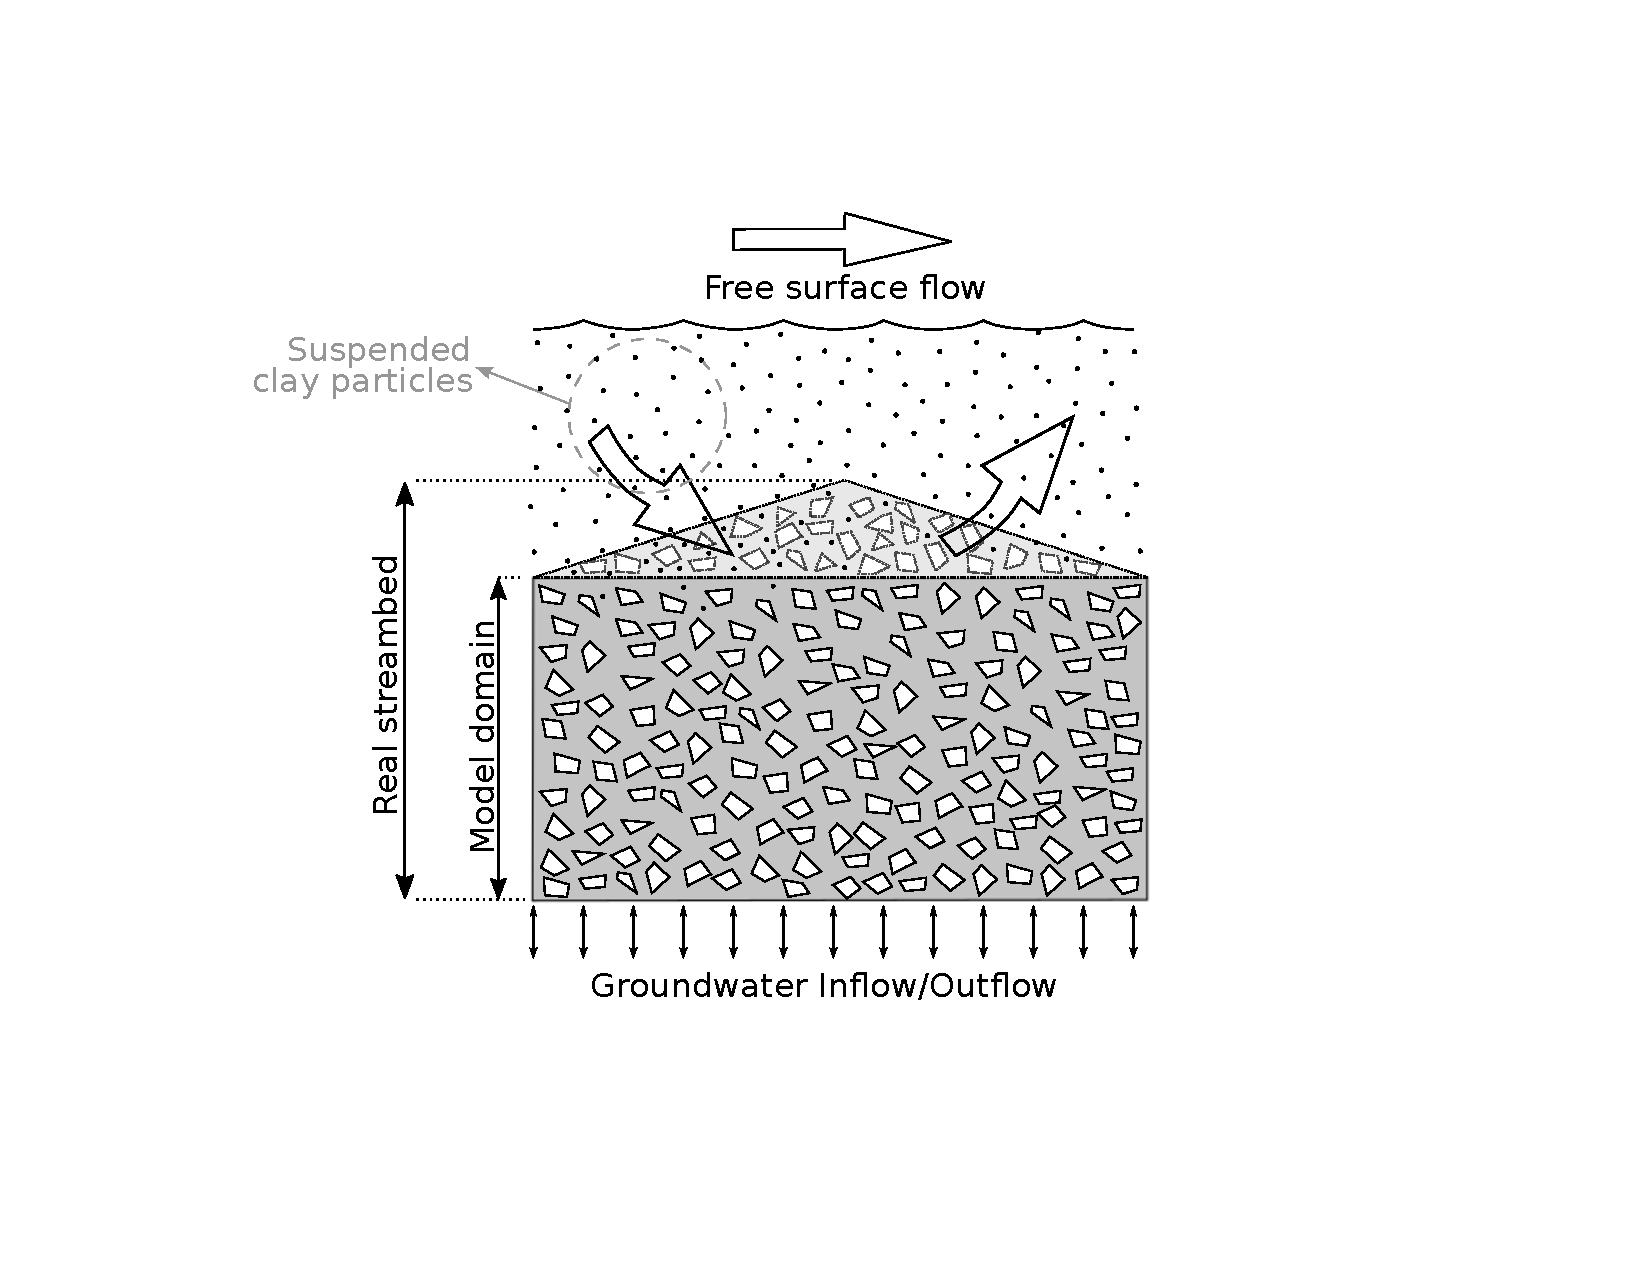
\includegraphics[clip, trim=4.2cm 4.5cm 8cm 3cm, width=18pc]
{1807010Conceptual.pdf}
\caption{Conceptual model for the posed problem}
\label{Conceptual}
\end{figure}
% ============================================================================

% ============================================================================
% TABLE WITH PHYSICAL AND NUMERICAL PARAMETERS FOR THE PARTICLE-TRACKING
% MODEL THAT WAS PROPOSED
% ============================================================================
\begin{table}
\caption{Physical \citep{Fox2018} and numerical parameters \citep{Packman2000}
for the particle-tracking model. }
\label{TF:Phys_Param}
\centering
\begin{tabular}{l c c}
\hline
PHYSICAL PARAMETERS						& SYMBOL			& VALUE			\\
\hline
  Flume width $[cm]$  					& $W$				& 29.0 			\\
  Sediment porosity $[-]$				& $\theta$			& 0.33 			\\
  Hydraulic conductivity $[cm/s]$ 		& $K$				& 0.12 			\\
  Flow $[l/min]$						& $Q$				& 261.0			\\
  Mean stream velocity $[cm/s]$			& $U$				& 15.0 			\\
  Streambed depth $[cm]$				& $d_b$				& 20.0 			\\
  Dune wavelegth $[cm]$					& $\lambda$			& 15.0 			\\
  Water depth $[cm]$					& $d$				& 8.8 			\\
  Total streambed area $[cm^{2}]$		& $A$				& 15.1	 		\\
  Inflow/Outflow$^{b}$ $[cm/d]$			& $q_{in}$			& $\pm 12.5$	\\
  Filtering coefficient $[1/cm]$		& $\lambda_f$		& 0.6			\\
\hline
NUMERICAL PARAMETERS					& 					& 				\\
\hline
  Number of particles $[-]$				& $n$				& 1.0E5			\\
  Real time simulated $[min]$			& $T$				& 60.0 			\\
  Number of timesteps per simulation $[-]$ &$nT$			& 1.0E4			\\
  Horzontal particle offset $[-]$		& $x_{off}$			& 1.0E-3		\\
  Vertical particle offset $[-]$		& $y_{off}$			& $100*eps^{c}$ \\
\hline
\multicolumn{2}{l}{$^{a}$All units in $cgs$ system for convenience} \\
\multicolumn{2}{l}{$^{b}$Positive quantities point upwards, negative 
downwards} \\
\multicolumn{2}{l}{$^{c}$Machine precision}
\end{tabular}
\end{table}
% ============================================================================

Our model simulates the water flow in one dune of the flume bed, since the main assumption is that the shape of the dunes and clay's behavior inside the dunes of the flume is fairly similar or repetitive, for the sake of simplicity \citep{Vanoni1974}. For our model, the shape of the dunes from \citet{Fox2014,Fox2018} were taken as a reference. 

\subsection{Mathematical Model} \label{Mathematical_model}

The velocity profiles used for modeling the water flow inside the dune are taken from existing literature \citep{Packman2000} and are illustrated in equations \ref{u} and \ref{v}. Here, $x$ and $y$ are the Cartesian coordinates reference axis, $k$ stands for the normalized dune wavelength $(2 \pi / \lambda)$ and $u$ and $v$ for the horizontal and vertical velocity components, respectively. 

% Velocity profile equations - From Packman et al. 2000
% use \nonumber if you want to split an equation in different rows and not number a row
\begin{eqnarray}
\label{u}
  u & = & -(kKh_{m}) \cos(kx) [tanh(kd_b)sinh(ky) + cosh(ky)] \\
\label{v}
  v & = & -(kKh_{m})\sin(kx) [tanh(kd_b)cosh(ky) + sinh(ky)] \pm q_{in/out} 
\end{eqnarray}

For the sake of simplicity, the model will take into account an instantaneous injection of particles at the top of the domain. Furthermore, the quantities are normalized according to the theory developed for flow and transport in sand beds \citep{Elliott1997,Packman2000}. As a result, equations \ref{u} and \ref{v} can be transformed in equations \ref{ustar} and \ref{vstar}. Figure \ref{Velocities} show the resulting velocity profiles that feed the particle-tracking model. 

% Dimensionless velocity profiles - From Packman with Elliott 
\begin{eqnarray}
\label{ustar}
  u^* & = & -\cos(x^*)[tanh(d_b^*)sinh(y^*) + cosh(y^*)]\\
\label{vstar}
  v^* & = & -\sin(x^*)[tanh(d_b^*)cosh(y^*) + sinh(y^*)] \pm q_{in/out}^*
\end{eqnarray}

The velocity component that corresponds to the settling velocity was neglected for this model since the Stokes number of the particle IS close to zero, thus particle will follow the streamlines of the velocity profiles generated by equations \ref{u} and \ref{v} \citep{Clark2009}. Equation \ref{STK} shows the calculation of the Stokes number for clay particles moving in porous media with representative length and velocity. 

% Stokes number calculation
\begin{equation}
 \label{STK}
 	Stk = \frac{\rho_p d_p^2 u_0}{18 \mu_f l_0} = \frac{2650 \frac{kg}{m^3} \cdot [384 \times 10^{-6}m]^2 \cdot 0.01 \frac{m}{s}}{18 \cdot 1.519 \times 10^{-3}Pa \ s \cdot 0.01 m} = 0.014
 \end{equation}

Where $\rho_p$ stands for the typical density of kaolinite \citep{NationalCenterforBiotechnologyInformation}, $d_p$ is the mean particle diameter \citep{Fox2014}, $u_0$ is the mean velocity, which is taken to be greater than the maximum obtained from equations \ref{u} and \ref{v}, $\mu_f$ is water's dynamic viscosity \citep{Cengel2006}, and $l_0$ is the characteristic length of the phenomenon which is similar to the dune height \citep{Fox2018}. The value of the stokes number is less than 1.0, i.e. a clay particle will follow the streamlines of the velocity profile without diverging from them \citep{Tropea2007}.

% ============================================================================
% Velocity profiles - figure
\begin{figure}[ht]
\centering
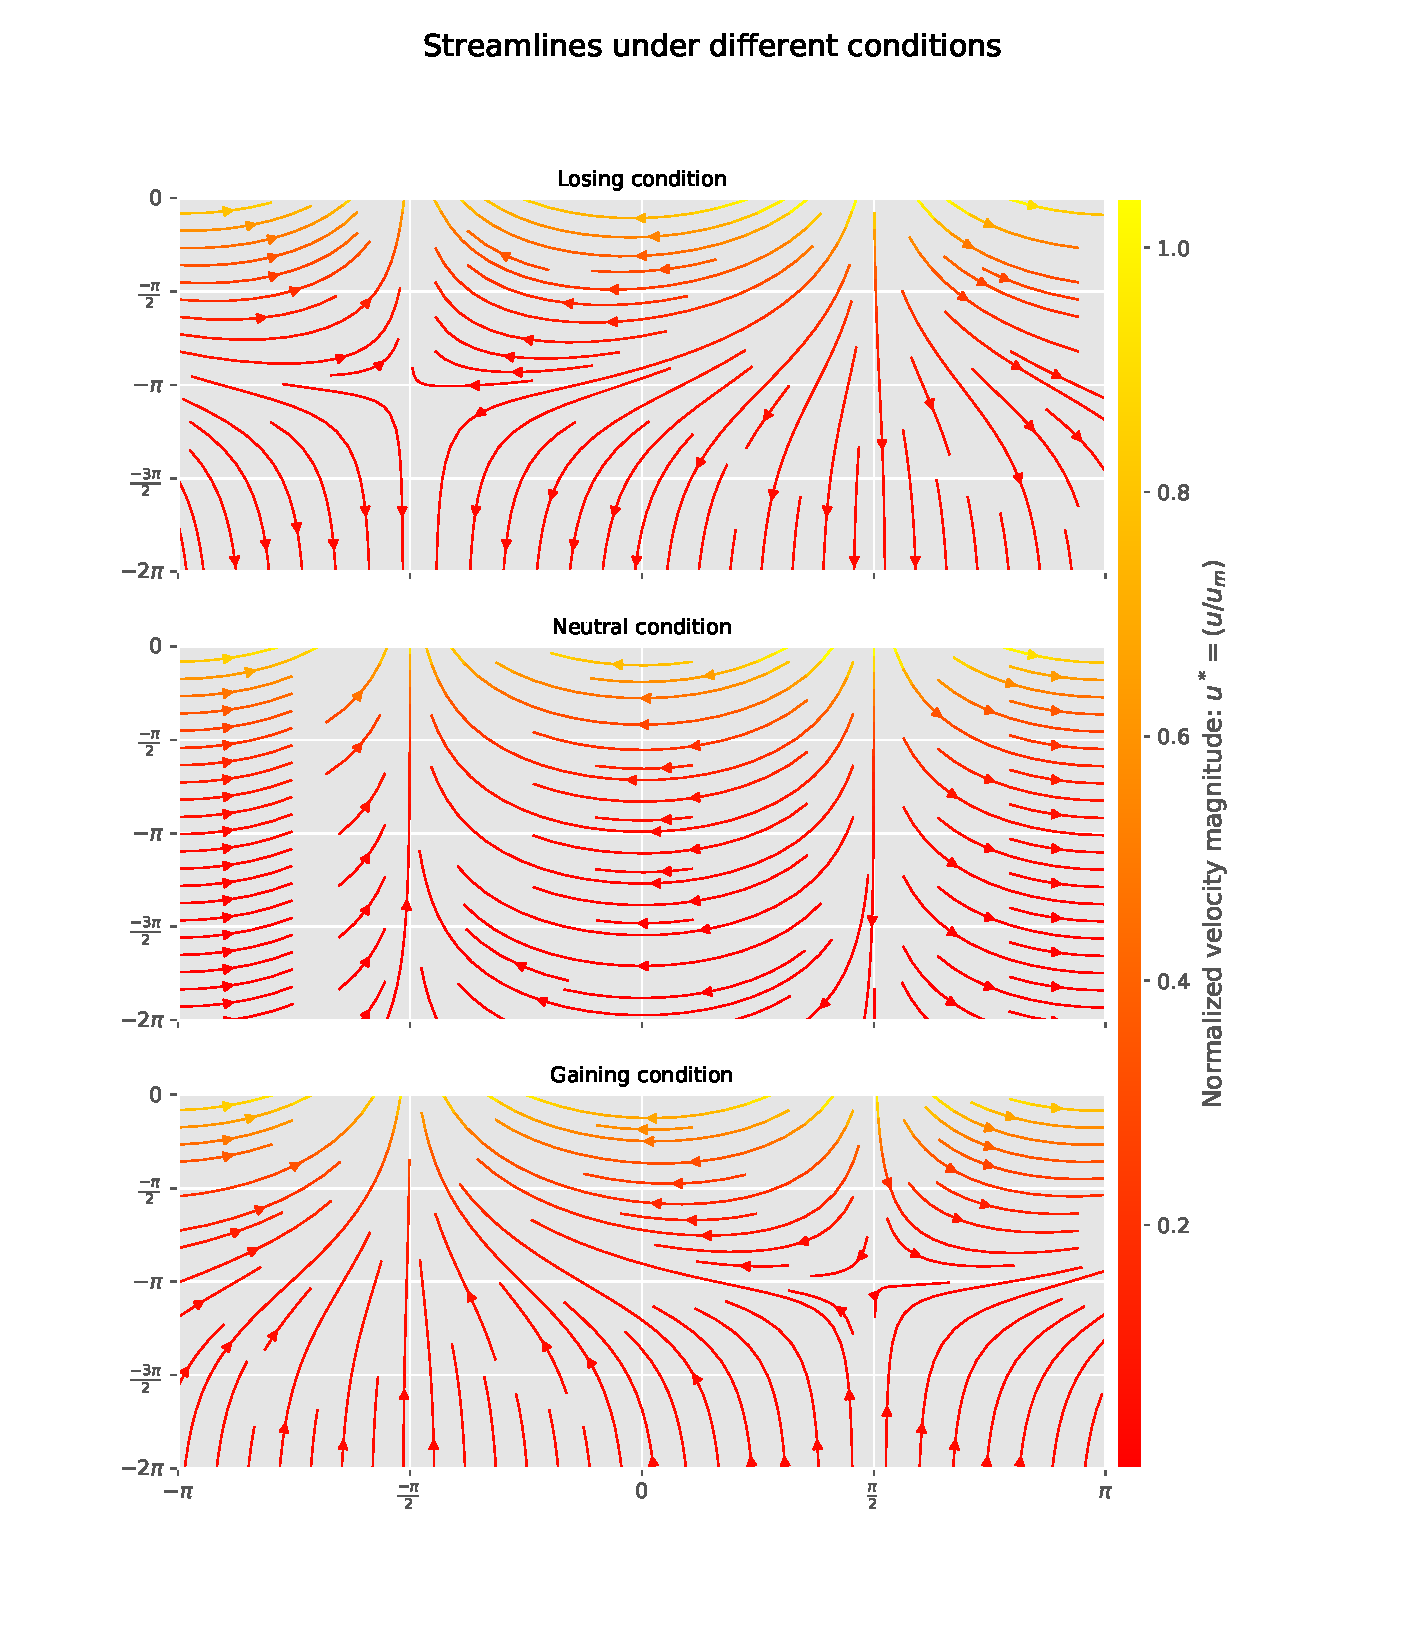
\includegraphics[trim=2cm 1.5cm 4cm 0.1cm, width=25pc]
{181203_Streamlines.pdf}
\caption{Streamlines under different vertical flow conditions: (A) Losing, (B) Neutral and (C) Gaining. Plots' domains are shifted from $[0, 2 \pi]$ to $[-\pi /2, \pi/2]$ since domain is periodic. Note that the vertical scale is distorted.}
\label{Velocities}
\end{figure}
% ============================================================================

The modeled clay particles follow the streamlines formed by the velocity profiles described in equations \ref{ustar} and \ref{vstar} they are not a solute, i.e. they don't take into account dispersive processes \citep{Domenico1998}. As a consequence, the particles' transport is composed by the advection caused by the velocity profile and the effects of filtration that have to be included as a stochastic process over each particle that is simulated at the end of every time step \citep{Prickett1981}. 

Consequently, the standard Advection Dispersion Equation is transformed into a transport equation that takes into account only the advection process as depicted in equation \ref{ADE}. Namely, in the continuum an advection process will move a concentration front with a given velocity profile. For the case of this research, the velocity profiles are the ones given in equations \ref{ustar} and \ref{vstar}.

% Advection Dispersion Equation with just advection!!!!
\begin{equation}
 \label{ADE}
 	\frac{\partial C}{\partial t} \ = -u \frac{\partial C}{\partial \bar{x}}
 \end{equation}

The second part of the model takes into account the filtration, which is modeled as a first-order process that depends on the path traveled by a particle, as shown in equation \ref{Filt_cont}. Where $\lambda$ denotes the filtration coefficient between 0.0 and 1.0, and $s$ the distance traveled by the concentration front. It is worth noticing that the proposed filtration process is independent of time. 

% Concentration reduction due to filtration of particles (equation)
 \begin{equation}
 \label{Filt_cont}
 	\frac{\partial C}{\partial s} \ = -\lambda C
 \end{equation}

\subsection{Numerical Model} \label{Numerical_model}

The numerical model proposed is shown in figure \ref{Numerical} and the initial conditions are shown in the bottom part of table \ref{TF:Phys_Param}. Its logical process is divided in three parts that use the discrete versions of equations \ref{ADE} and \ref{Filt_cont}. These versions have been proposed in the literature \citep{Delay2005,Dentz2011}, following a modified version of the Langevin equation, suited to represent in a discrete way the ADE. The first step takes into account the initial position of each particle and calculates the displacement of particles using equations \ref{dispx} and \ref{dispy} \citep{Li2017}. Hence, each timestep the model takes into account the position of each particle and interpolates the velocity fields to determine each particle's velocity at the point where it is. It is worth noticing that collision between particles is not taken into account for the sake of simplicity of the model. 

% ============================================================================
% Numerical model of the problem proposed - figure
\begin{figure}[ht]
\centering
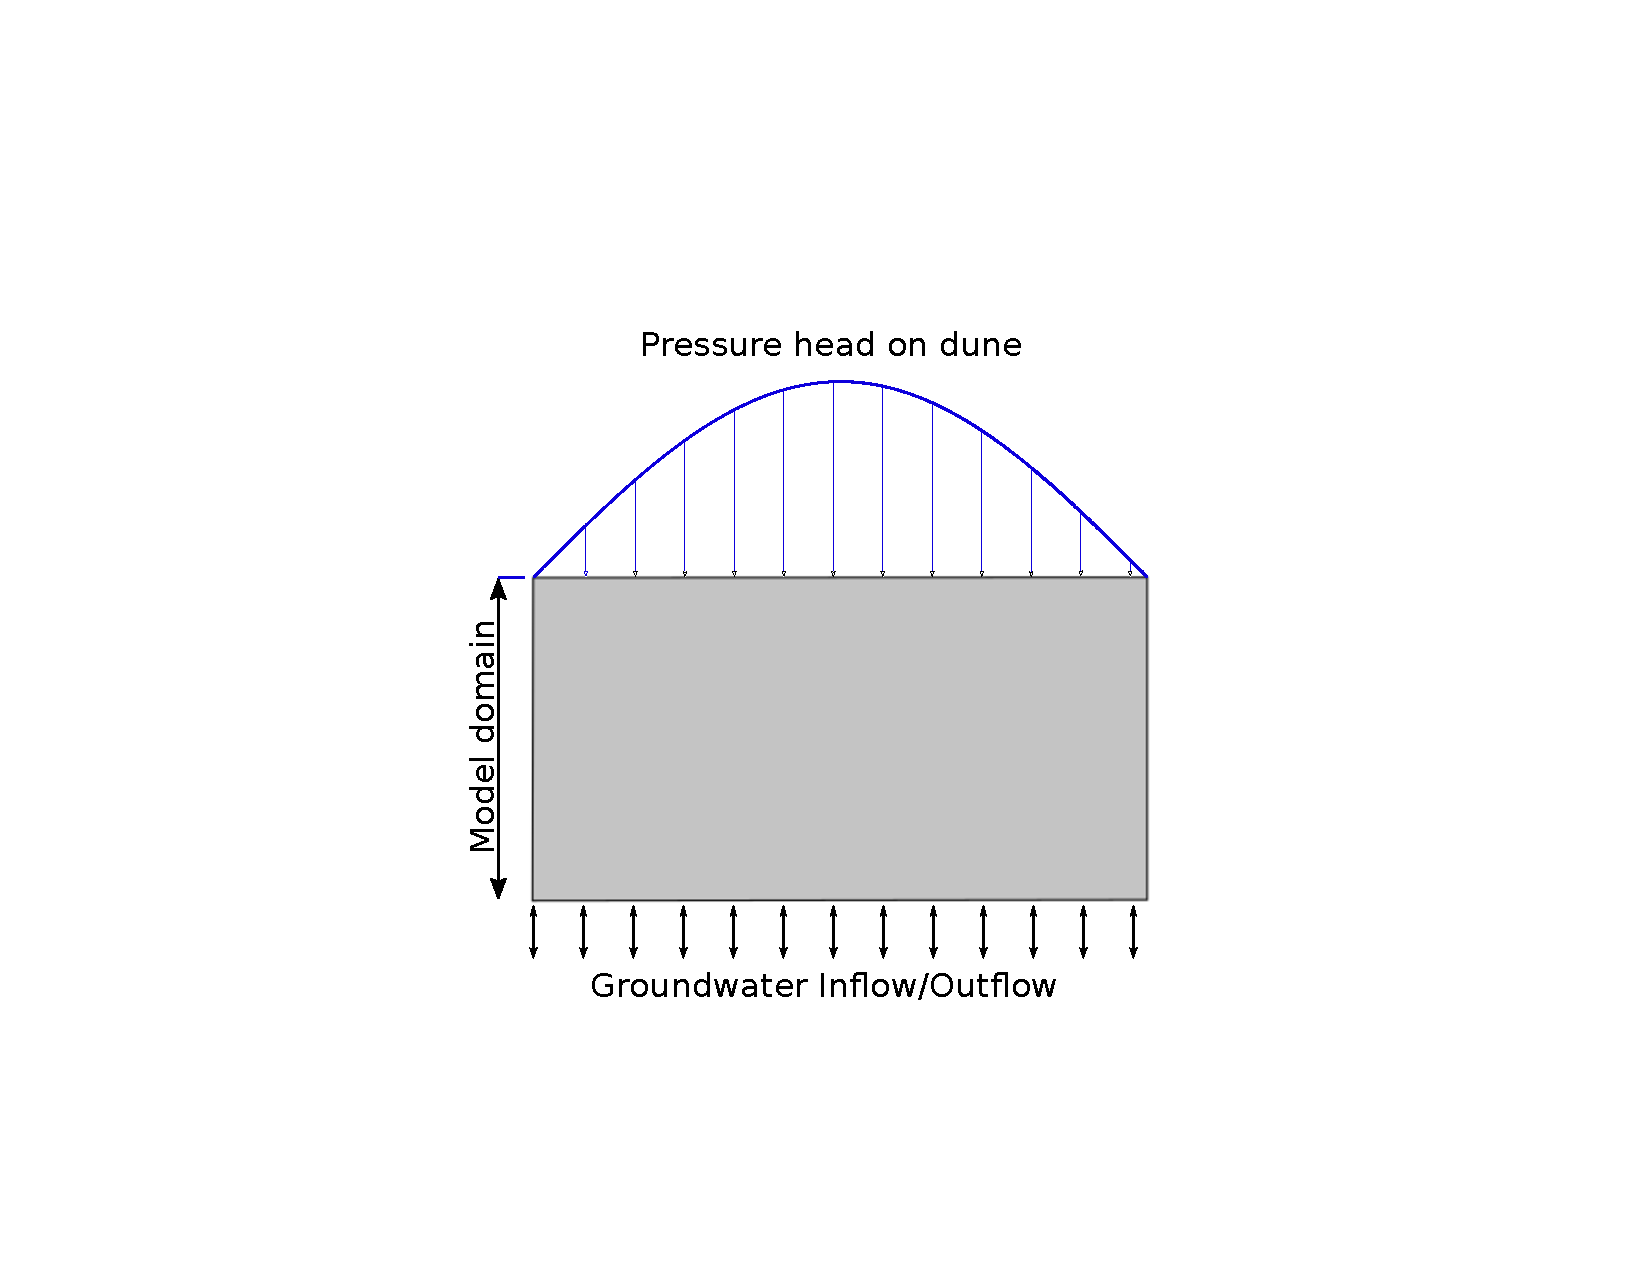
\includegraphics[clip, trim=4.2cm 4.5cm 8cm 3cm, width=18pc]
{181129Numerical.pdf}
\caption{Depiction of numerical model proposed}
\label{Numerical}
\end{figure}
% ============================================================================

% Particle displacement for the "first step" of the numerical model
\begin{eqnarray}
 \label{dispx}
 	x(t + \Delta t) = x(t)  + u \cdot \Delta t\\
 \label{dispy}
 	y(t + \Delta t) = y(t) + v \cdot \Delta t
 \end{eqnarray}
 
In non dimensional form, the displacement is:

% Particle displacement for the "first step" of the numerical model
\begin{eqnarray}
 \label{dispx_s}
 	x^*(t^* + \Delta t^*) = x^*(t^*)  + u^* \cdot \Delta t^*\\
 \label{dispy_s}
 	y^*(t^* + \Delta t^*) = y^*(t^*) + v^* \cdot \Delta t^*
 \end{eqnarray}
 
After estimating each particle's position, the discrete filtration process is modeled using a uniform random number generator inside the script. To do so, the filtration coefficient is taken as each  particle's probability of being filtered given that it traveled certain  distance. Therefore, equation \ref{Filt_cont} is translated to the discrete domain using equation \ref{Filt_disc}, since the timestep size is small enough to hold the relationship posed in the right hand side of equation \ref{Filt_disc} \citep{Li2017}.
 
 % Simplification of the continuum - from eulerian to particles
 \begin{equation}
 \label{Filt_disc}
 	p = 1 - e^{-\lambda_f ds} \approx \lambda_{f} ds
 \end{equation}

Finally, the third part of the model consists of counting the amount of particles that are still in the domain, which is divided in filtered particles that will remain still for the rest of the simulation; and moving particles, which have not been filtered yet. Moreover, the model accounts for the particles that went out of the domain because of the remobilization process. Particularly, the particles that are remobilized every timestep are not allowed to come back to the model any more. 

To ensure that the computational domain of the model is representative of a single dune, the boundary conditions at the right and left walls of the model are periodic. Namely, a particle that has an $x^* < 0$ will appear at the right of the domain. Correspondingly, a particle's $x^* > 2 \pi$ is transferred to the left part of the domain. Regarding the bottom boundary, any particle whose $y^* < d_b^*$ bounces inside the domain. On the other hand, any particle whose $y^* > 0$ is counted as remobilized and exits the simulation. 

The particle-tracking simulations were performed under similar conditions to the ones proposed in table \ref{TF:Phys_Param} with $1e^5$ particles for each vertical flow condition imposed (Losing, Neutral and Gaining). The total time simulated ensured that all of the seeded particles were remobilized of filtered at the end of the simulation. Nonetheless, the clay injection proposed in the numerical model is instantaneous and not continuous as in the experimental set-up. 

As regards to the initial condition, the particles are seeded evenly distributed at the top of the domain and just in the left portion of it ($0 < x^* < \pi$), since particles seeded at the right part of the domain ($\pi < x^* < 2\pi$) will immediately be remobilized due to the velocity profiles provided for the particle flow, as shown in figure \ref{Velocities}. At the end of every simulation, the results are two tables with coordinates of filtered and moving particles for every timestep, and a vector that counts the remobilized particles in the different timesteps. 

% About the relative concentration windows where the results are analyzed.
These raw results are then grouped to get information that is comparable with experimental results. Hence, the model's domain is divided into squares with $\pi / 100$ side and then particles are counted every timestep recorded to get the relative concentration in the grid of the model. The domain division is independent from the interpolation points used for the velocity interpolation. 

Selecting the mesh size for the particle counting is not trivial and in this case, different sizes of mesh were tested. If the mesh is coarse, the results will not be able to represent the phenomenon, and if the mesh size approaches to zero, the number of particles in every cell will not be representative of the phenomenon that is being modeled \citep{Xue2017}. In addition, methods like kernel density estimation (KDE), are not explored here since this is not the scope of this research. 

% ================================================================================
% RESULTS SECTION
% ================================================================================
\section{Results}  \label{Results}

% 0. VELOCITY PROFILES UNDER DIFFERENT CONDITIONS WHEN SOLVING FOR THE DIFFERENT IN/OUT VALUES
The velocity profiles that result from equations \ref{ustar} and \ref{vstar} that are shown in figure \ref{Velocities} show substantial differences among them. Indeed, there is a preferential flow going upwards or downwards if the imposed condition is a gaining or losing flow, respectively. Furthermore, there is a no flow zone in the losing and gaining conditions formed by the addition of a vertical flow to a neutral flow condition. Consequently, there is a recirculation zone in the losing and gaining cases, though they are in different places according to the case. For instance, in the gaining condition it is located in the right part of the domain, while for the losing condition it is located at the left.

Furthermore, the maximum velocity in each profile is located in a different place. Namely, in the losing condition the maximum velocity is in the negative direction at the stoss side of the domain, while in the gaining case it is located in dune's lee. However, for the neutral condition there are two maximum velocities, one located in the stoss and the second in the lee. These features that the velocity profiles exhibit are key to understand the deposition of particles inside the domain when running the PT model, and they are the responsible of the different deposition patterns that result.   

% 1. PARTICLE DEPOSITION OVER DIFFERENT TIMES AND DIFFERENT CONDITIONS (COMPARE BETWEEN THEM) - explain the plots
Both, the horizontal and the vertical extents of the particle deposition are dependent on the vertical flow conditions that are imposed to the numerical model. In fact, figure \ref{Heatmap} shows that the horizontal expansion of the clay deposition is different between the analyzed cases. Besides, the maximum depth of the clay in all of the times is different between the conditions modeled, as seen in the experimental results used for comparison. Nevertheless, a particular feature arises near the last quarter of the domain, where a gap is formed and no particles are present even at the top of the domain. This position marks the place where particles go out of the domain and are remobilized to the free surface flow. 

In addition, a perceptible difference between particles' deposition can be spotted when analyzing the width the gap formed between the places where particles are deposited. This result is clearly linked to the shape of the velocity profiles and marks the place where particles that are remobilized go out of the domain to the free stream flow. Figure \ref{Heatmap} shows that this gap is different in size according to the conditions that are being modeled. Namely, for the losing condition the gap is narrow, and it tend to stretch in neutral and gaining conditions. 

% ============================================================================
% Concentration map - figure
\begin{figure}[ht]
\centering
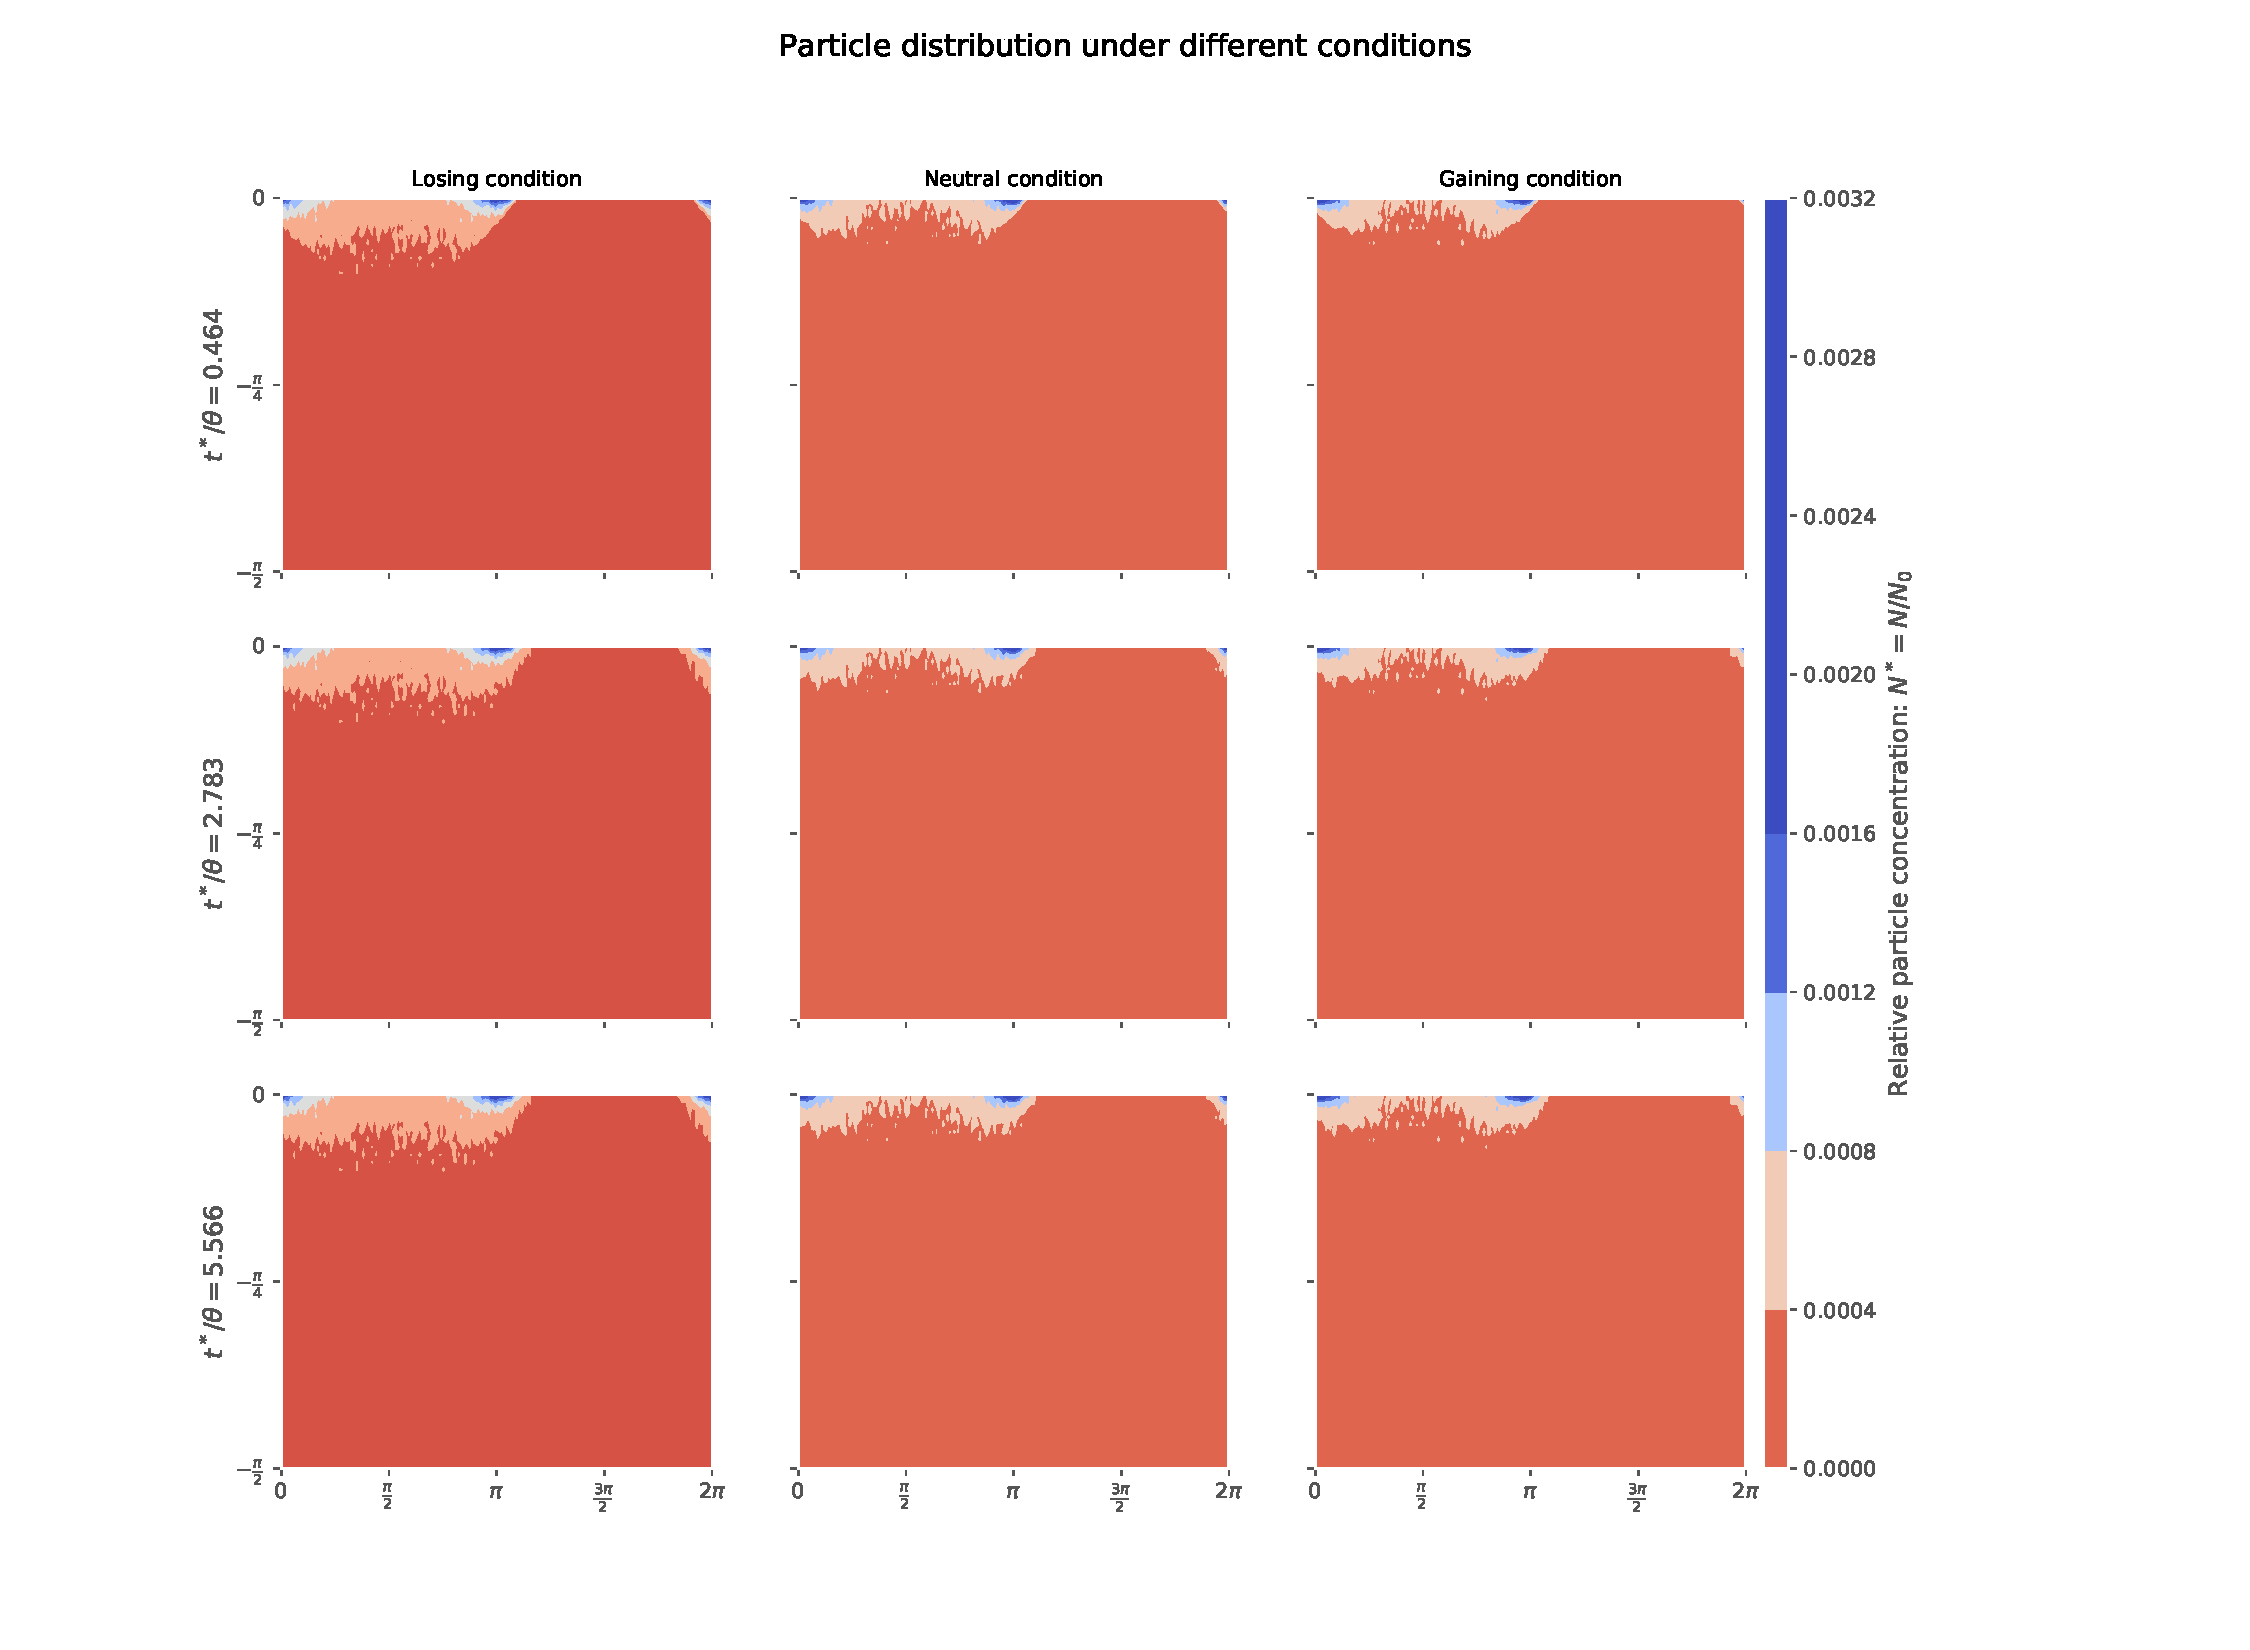
\includegraphics[trim=0.2cm 0.2cm 0.2cm 0.2cm, width=45pc]
{181203_Concentrations.pdf}
\caption{Particle deposition in different times (rows), and under different inflow/outflow conditions (columns) (Note that axis are not to scale).}
\label{Heatmap}
\end{figure}
% ============================================================================

% Logmap and how more differences can be spotted using this "lens"
However, the results shown in figure \ref{Heatmap} are similar in some ways and the differences between vertical flow conditions are greater in the experiments \citep{Fox2018}. To ease the results' analysis it is worth to present the results of figure \ref{Heatmap} in logarithmic scale. Figure \ref{Logmap} shows the particles' concentration at the top of the domain, just as the concentration maps in figure \ref{Heatmap}. Nevertheless, the logarithmic scale shows that the deposition of particles inside the domain has more differences between the inflow/outflow cases modeled. First of all, the gap that was shown in figure \ref{Heatmap} is more pronounced in the gaining condition than in neutral and losing conditions. 

Besides the gap, the logarithmic plot containing the number of particles shows that for the losing condition the amount of particles is more even at the top of the domain than for the neutral and gaining conditions. Besides, the width of the blue strata that shows more than $10^2$ particles is consistent only i9n the losing condition, while it tends to get thinner in the neutral condition and even tends to disappear for the gaining flow condition.

Figure \ref{Logmap} also shows the presence of spots with no particles. Namely, for the losing condition these spots are located at the bottom of the figure and tend to be more spread than for the neutral and gaining conditions. In fact, in the latter the presence of these spots is shown even at the top of the domain close to the gap discussed in figure \ref{Heatmap}. In particular, particle presence in the domain is fostered by the losing condition, and on the other hand it is hindered by the gaining condition. As a consequence, the gaining and neutral conditions have more spots with no particles than the losing condition, which tends to fill the whole upper part of the domain.

% ============================================================================
% Logarithm of concentration - figure
\begin{figure}[ht]
\centering
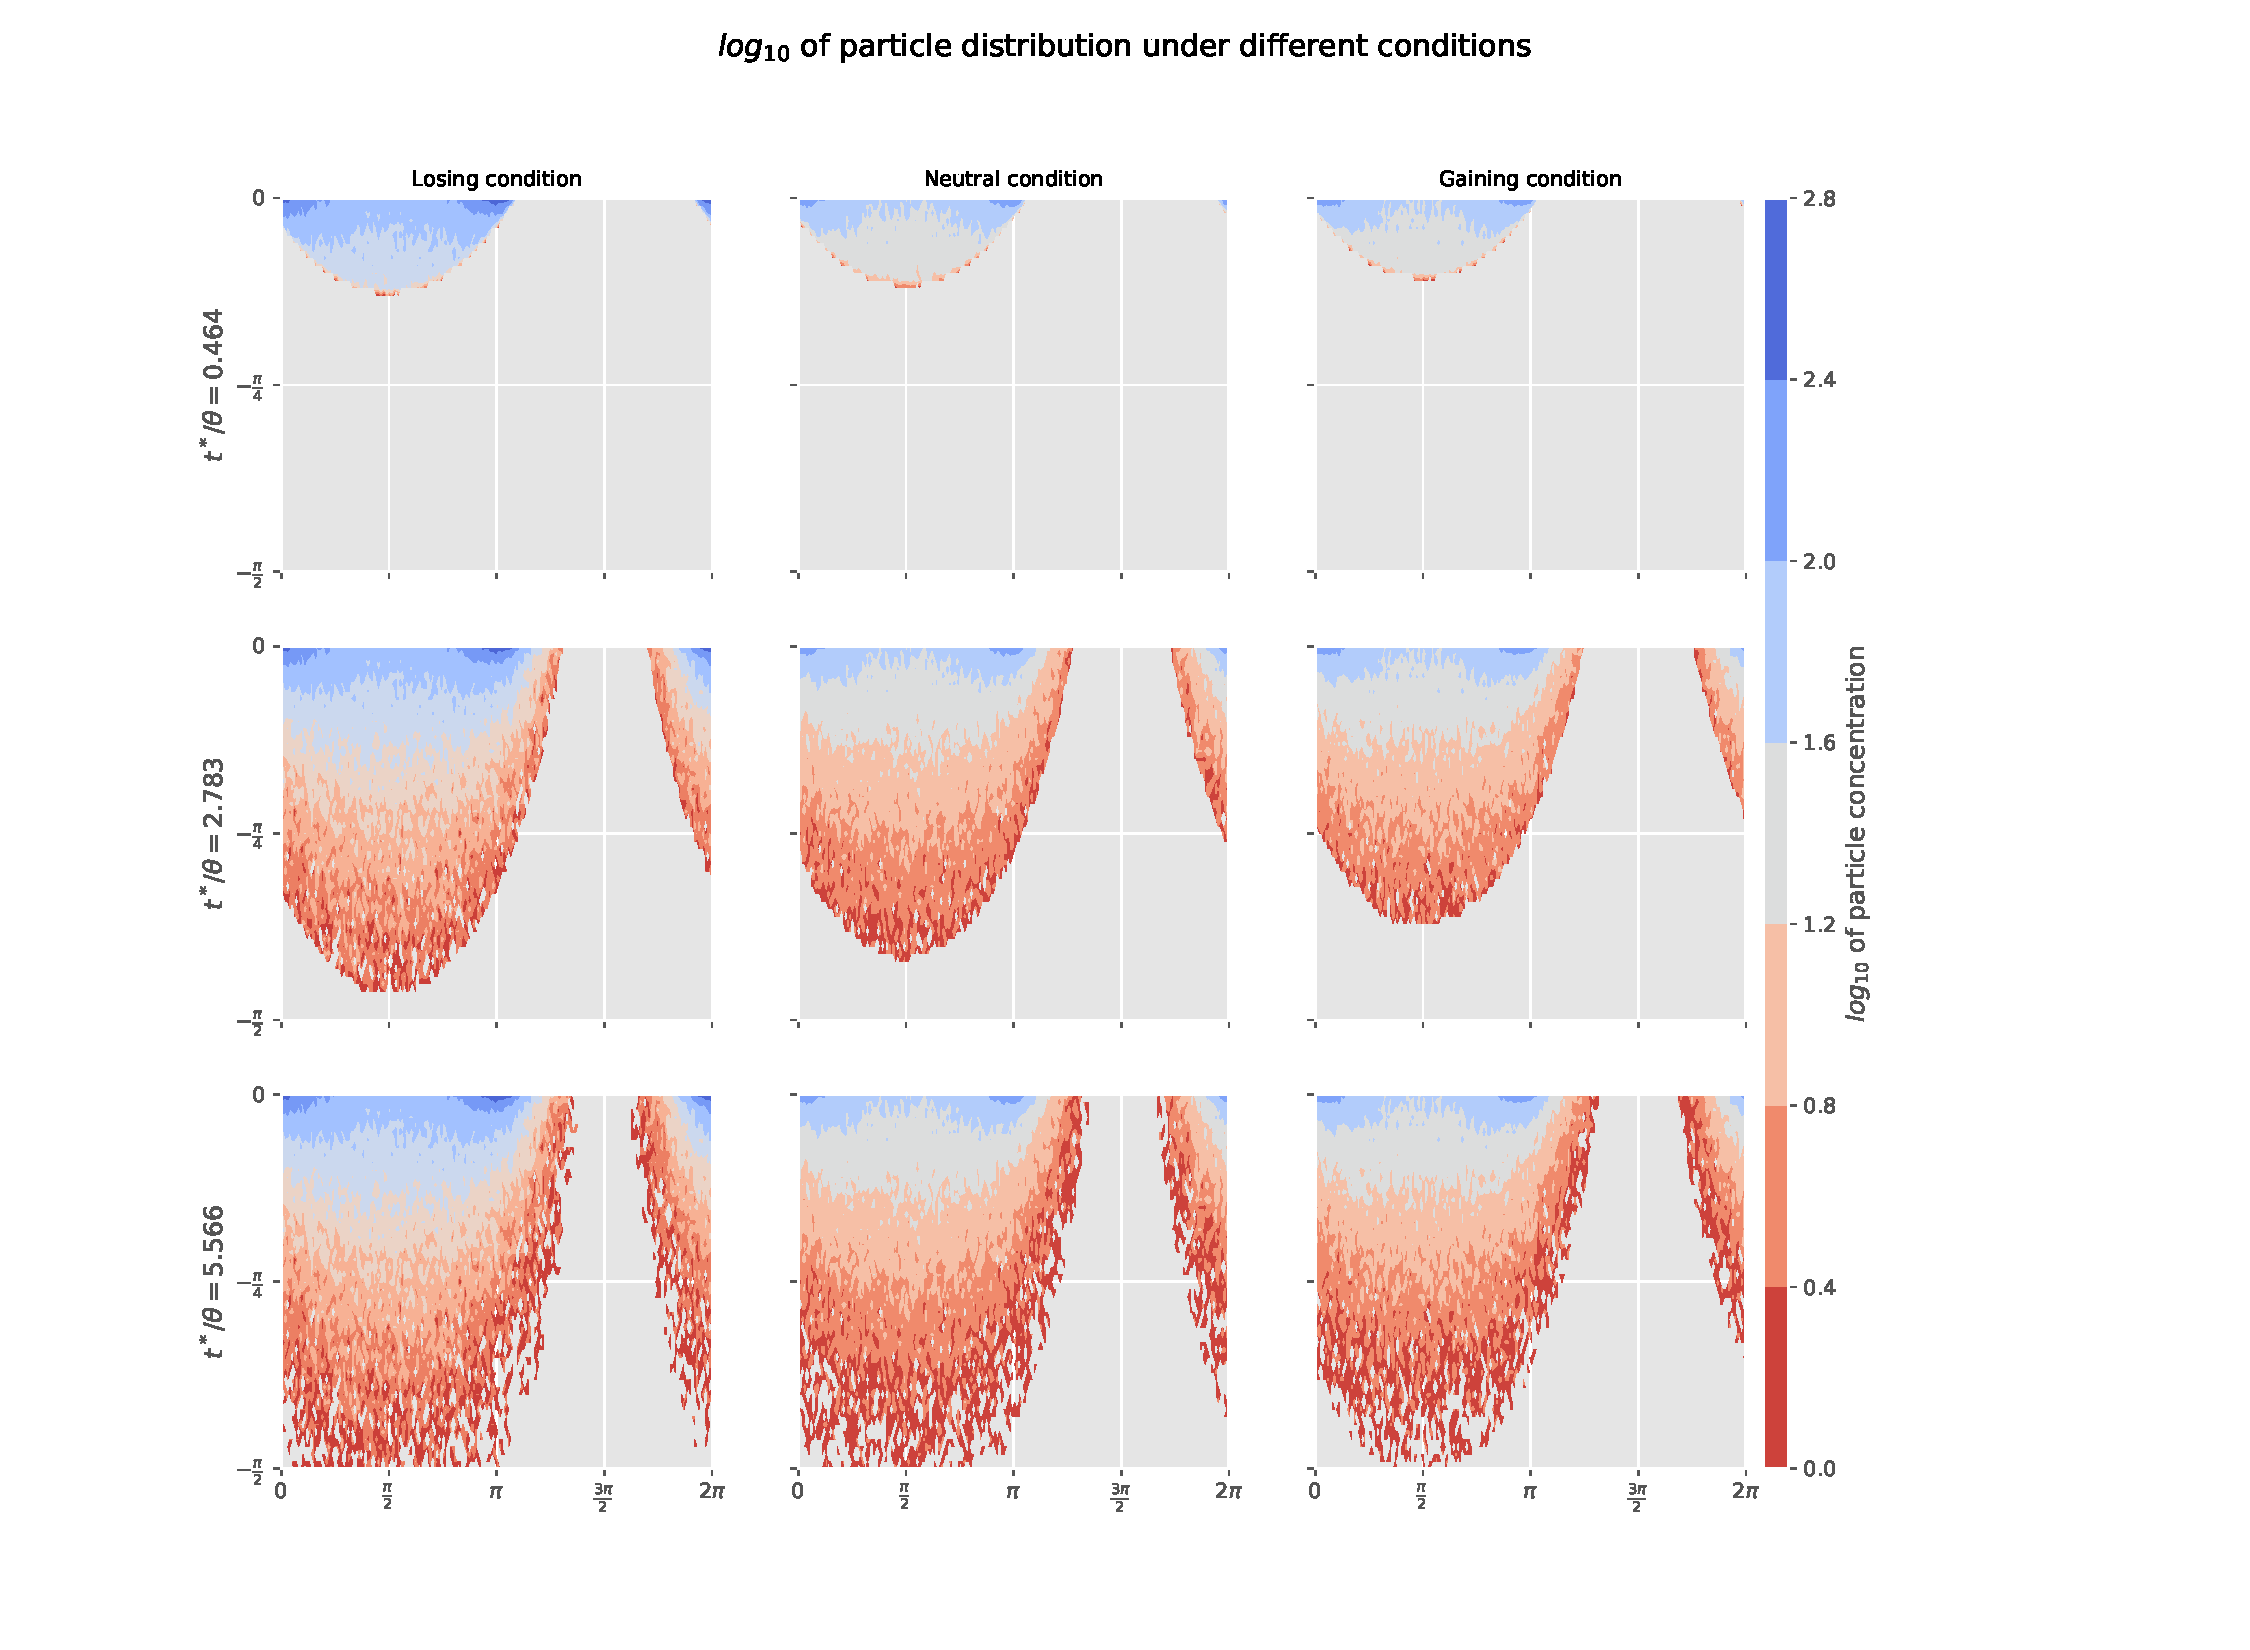
\includegraphics[trim=0.2cm 0.2cm 0.2cm 0.2cm, width=45pc]
{181203_Logplot.pdf}
\caption{Logarithm of particle deposition in different times (rows), and under different inflow/outflow conditions (columns) (Note that axis are not to scale).}
\label{Logmap}
\end{figure}
% ============================================================================

% 2. BEHAVIOR OF PARTICLES' IN TIME - HOW THEY GET DEPOSITED AND REMOBILIZED IN TIME ACCORDING TO THE FLOW CONDITIONS
Regarding the behavior of particles over time, figure \ref{Pvst} shows the relative number of particles that are moving inside the domain (blue line), filtered (purple line) and remobilized to the surface (red line). In particular, figure \ref{Pvst} shows that the even with identical filtering coefficients, the amount of particles that remain in the domain and that are remobilized varies significantly betwixt vertical flow conditions imposed.

% ============================================================================
% Particles in time - figure
\begin{figure}[ht]
\centering
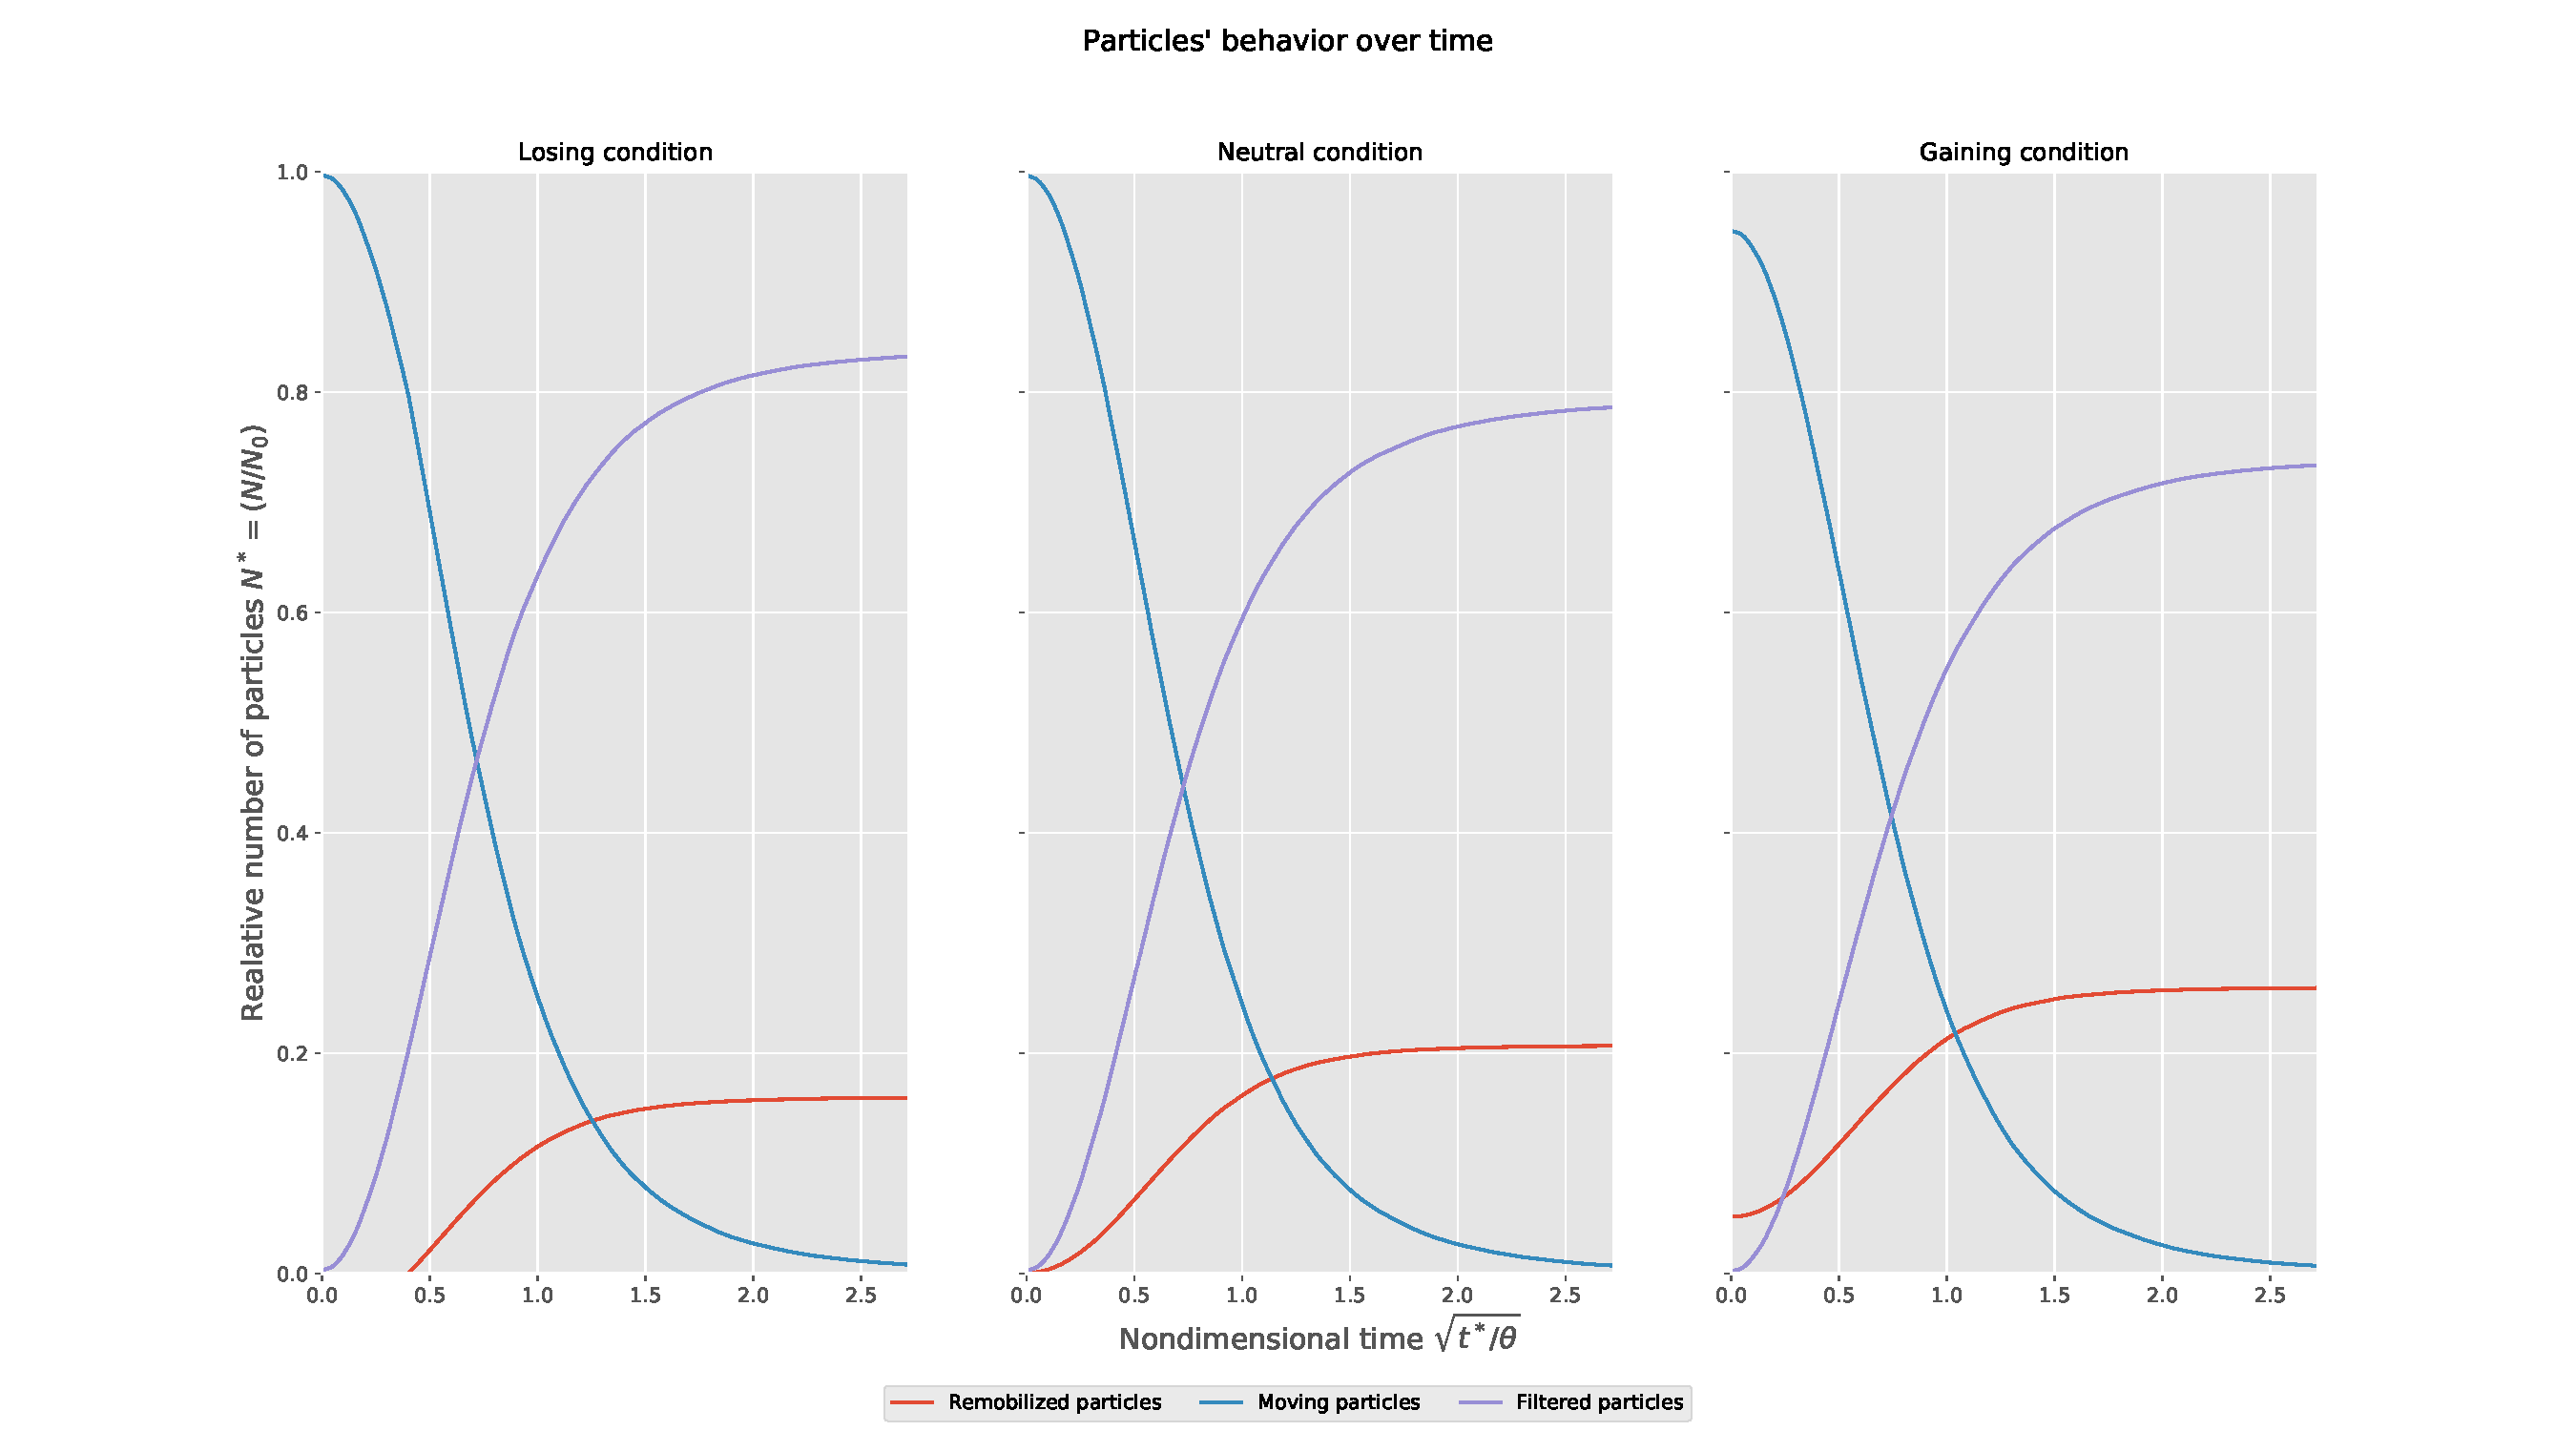
\includegraphics[trim=0.2cm 0.2cm 0.2cm 0.2cm, width=35pc]
{181203_Pvst.pdf}
\caption{Particle's behavior over time. A. Losing condition. B. Neutral condition and C. Gaining condition}
\label{Pvst}
\end{figure}
% ============================================================================

In respect of the moving particles in the domain, it is clear that they decrease in an exponential shape because of the filtering process that is occurring during the time of the simulation in the three modeled scenarios. Indeed, this decrease corresponds to the exponential decrease that results from solving equation \ref{Filt_cont} in a typical filtration problem. Nevertheless, the particles' decrease rate in the domain is different between the different vertical flow conditions showing that the filtering process is fostered or hindered by losing and gaining conditions, respectively. 

In the same way, the number of remobilized particles behaves according to the vertical flux imposed to the model. Therefore, as the flux increases positively (upwards), the number of remobilized particles increase respect to conditions with no vertical or negative (downwards) flux imposed. Distinctly, the number of remobilized particles is high at early times and it decreases as the simulation time goes by, rather than staying constant in time. 

On the subject of filtered particles, figure \ref{Pvst} shows that vertical flow conditions affect their presence inside the model's domain. In fact, the losing condition fosters the presence of filtered particles, while gaining flow condition hinders it. These results also work in the sense of checking that the sum of filtered. moving and remobilized particles at any time are the total number of particles seeded at the beginning of the simulation. 

% 4. RESIDENCE TIME AND PORTION OF PARTICLES INSIDE THE DOMAIN AT ANY GIVEN TIME.
Besides particles' location in space and time, the PT model can estimate the Residence Time Function (RTF). This feature points the fraction of mass that is present inside the stream bed after and injection performed in a given time $t_0$ \citep{Elliott1997,Packman2000}. Therefore, dividing the the sum of filtered particles and moving particles inside the domain by the total number of particles seeded at every timestep will result in the RTF of the PT model. Figure \ref{RTF} shows the RTF for the three vertical flow conditions modeled.

% ============================================================================
% Residence time function - figure
\begin{figure}[ht]
\centering
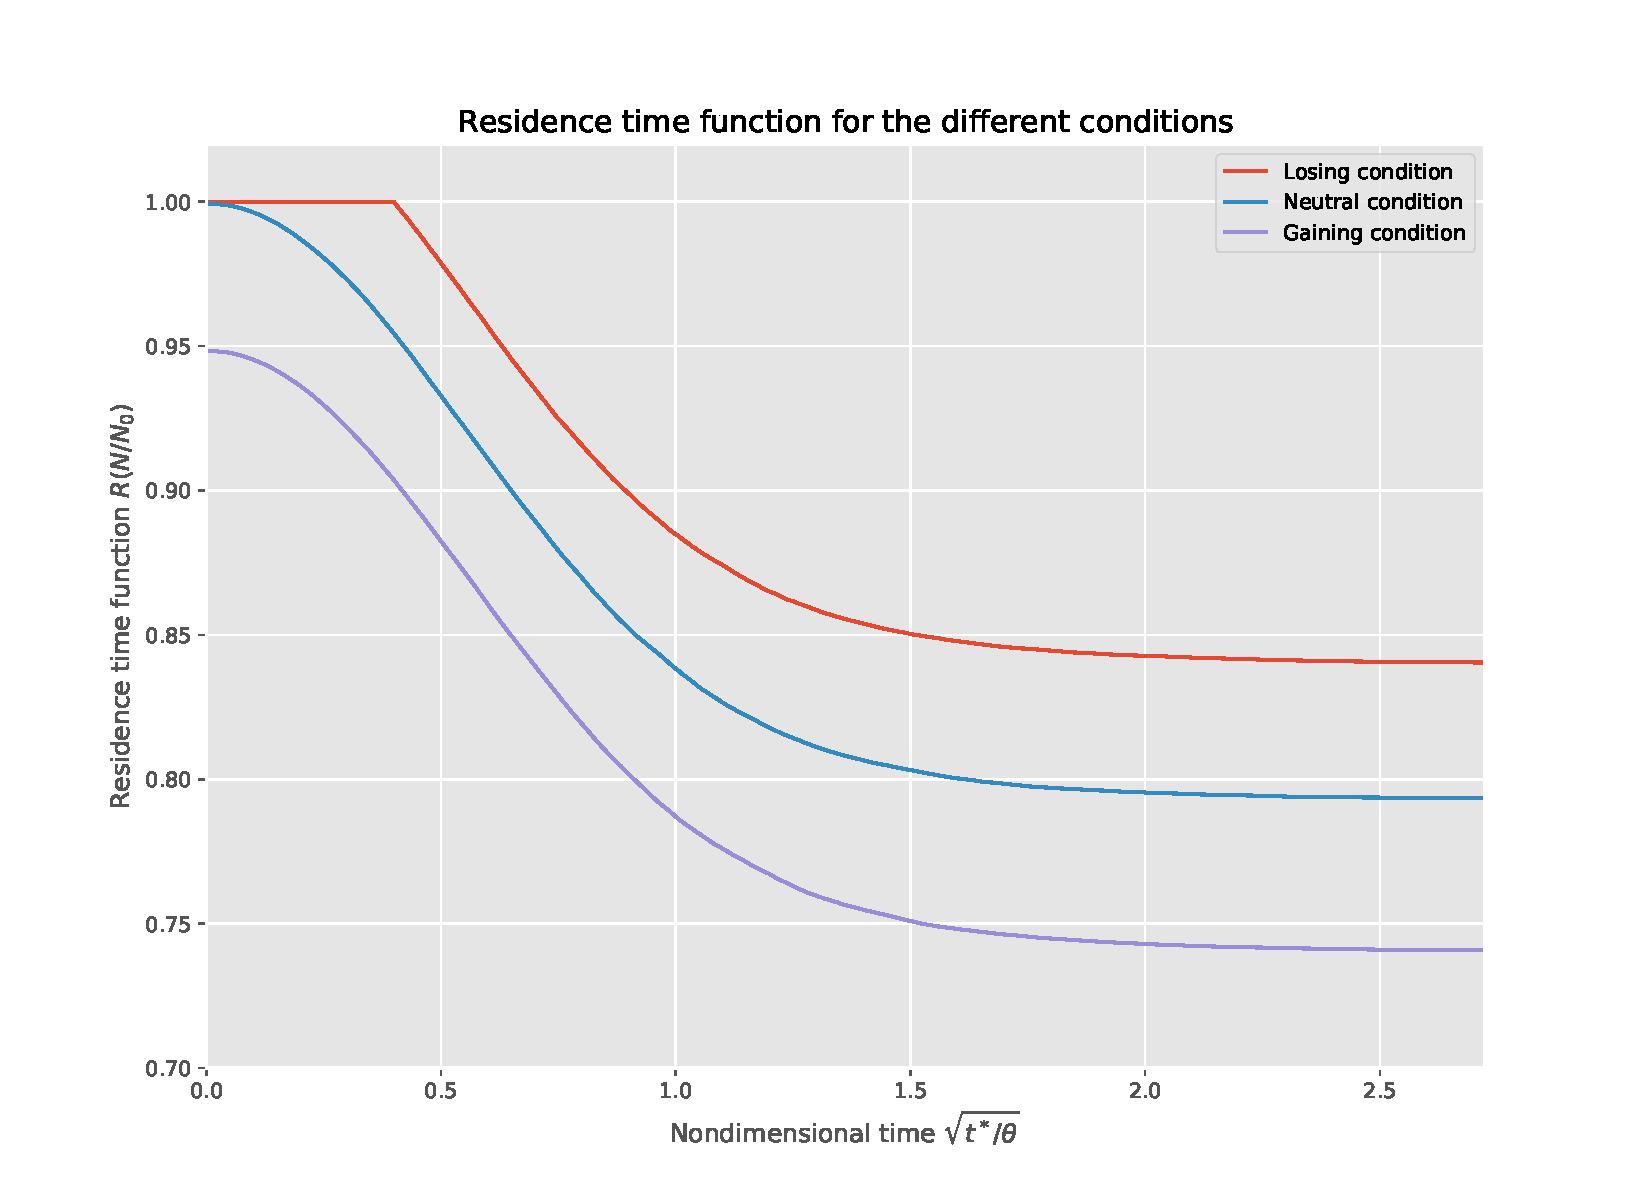
\includegraphics[trim=0.2cm 0.2cm 0.2cm 0.2cm, width=20pc]
{181203_RTF.pdf}
\caption{Residence time function for different flow conditions imposed}
\label{RTF}
\end{figure}
% ============================================================================

% 5. Residence time function and the derivative (check when the othe rmodel is run)
The first interesting feature about figure \ref{RTF} is that some of the particles will remain in the bed indefinitely since they have been filtered by the model. Nevertheless, the amount of particles inside it is clearly affected by the vertical flow conditions imposed, since more particles are retained in the bed in the losing condition than in the neutral or in the gaining condition. Furthermore, the RTF is not constant until late times, showing that filtration and vertical flow conditions affect hyporheic exchange in different ways according to the model conditions imposed.   

Since the gaining and losing conditions are symmetrical, the expected results of the RTF for the losing and gaining conditions are expected to be equally distant from the RTF curve of the neutral condition. Nevertheless, figure \ref{RTF} shows that this is not the case. Actually, the losing condition RTF is closer to the neutral condition than the gaining one. To explore this, figure \ref{RTFder} shows the rate of change of the RTF in time for the three cases.

% ============================================================================
% RTF der - figure
\begin{figure}[ht]
\centering
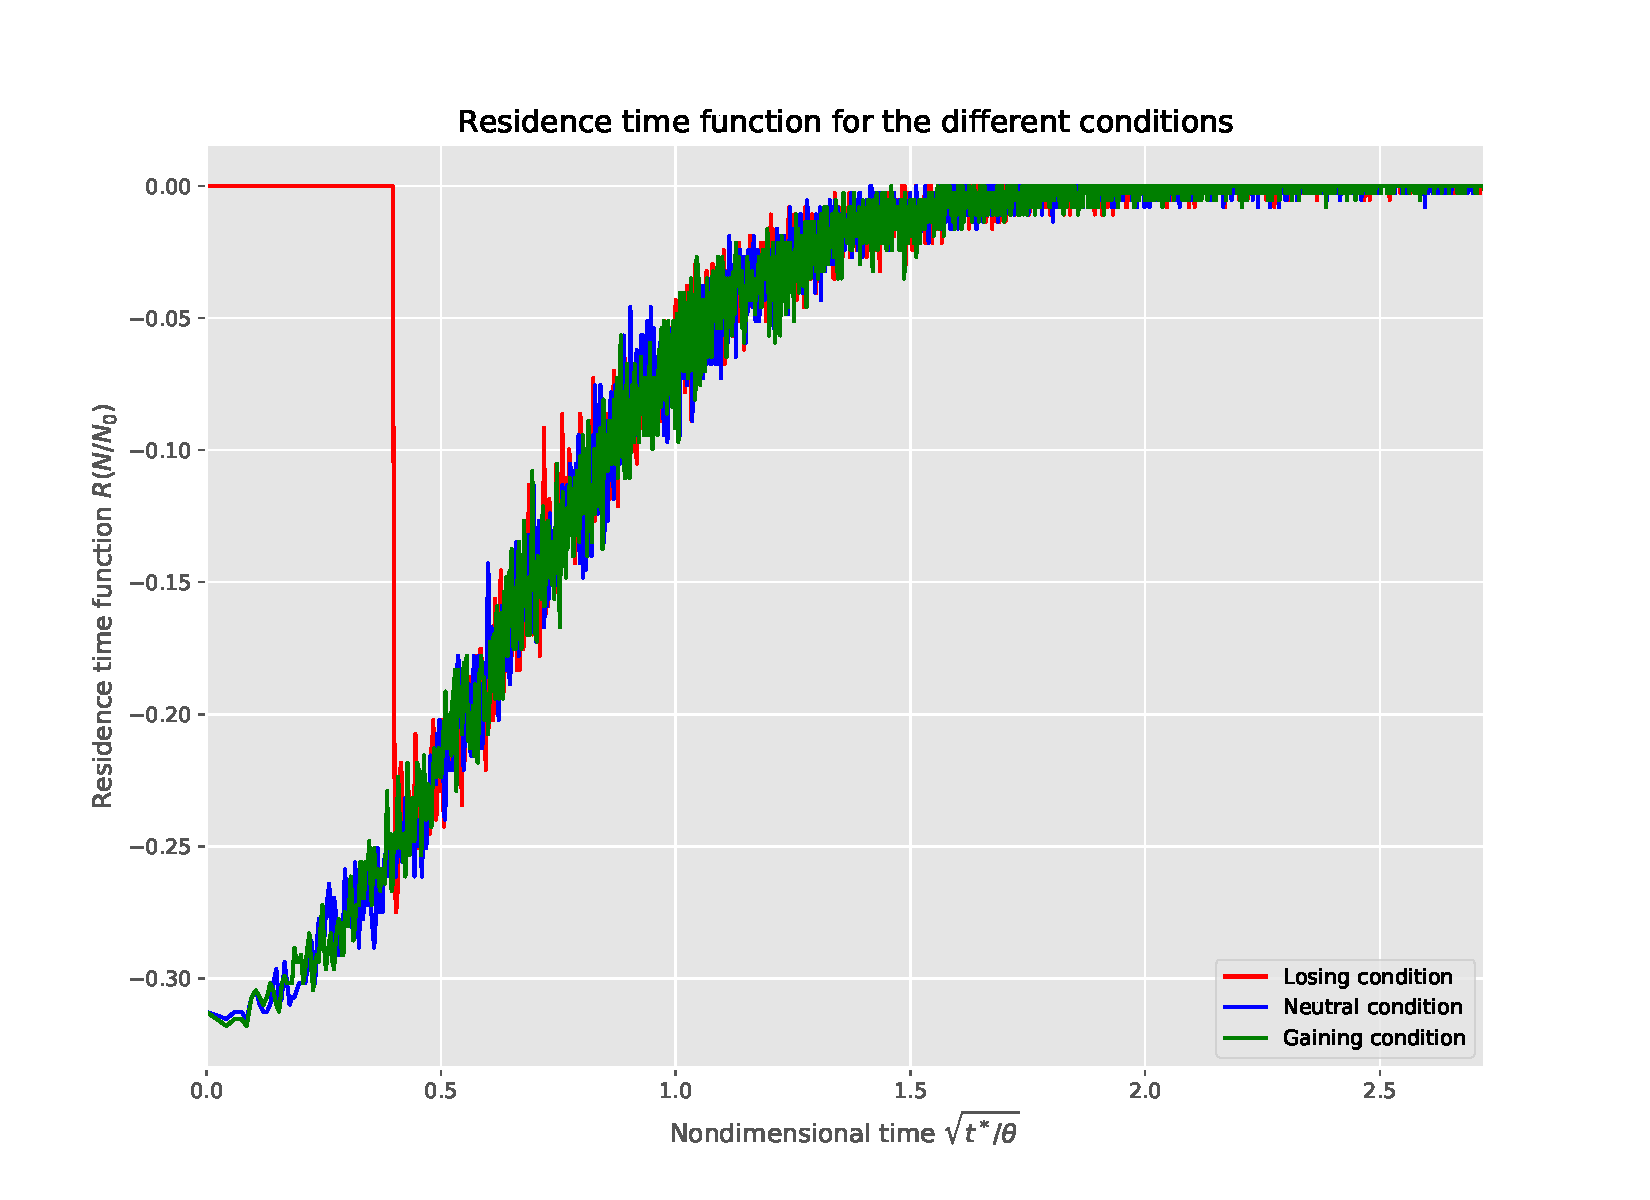
\includegraphics[trim=0.2cm 0.2cm 0.2cm 0.2cm, width=20pc]
{181203_RTF_der.pdf}
\caption{Derivative of RTF for the three conditions}
\label{RTFder}
\end{figure}
% ============================================================================

In addition, figure \ref{Pvst} shows that for the losing condition all of the particles stay inside the domain for a small time and later they start remobilizing, thus the RTF is constant at early times and starts to change after certain time that corresponds to the minimal path that a particle can travel through the domain. This feature is also shown in figure \ref{RTFder}, where the red line (losing condition), starts with a derivative equal to 0.0 and suddenly jumps to start varying. 

Figure \ref{RTFder} shows the rate of change in time of the RTF for each one of the three cases modeled. It is evident that for almost any time, the rate of change of particles inside the domain is the same for the three modeled cases. Nonetheless, there is a delay for the losing condition (red line), where all the particles remain inside the domain at early times and start to change later than in the other two modeled cases.

Even so, the three RTF shown in figure \ref{RTF} stop changing after a certain time since all of the particles of the domain have been filtered or have left the domain due to remobilization. Moreover, the fraction of mass remaining inside the domain after any time $t^*/\theta$ is different for each one of the vertical flow conditions modeled. 

Regarding the decrease of particles inside the domain, figure \ref{MOVder} the change of moving particles inside the domain with time. These results show clearly that the rate of removal of particles (due to remobilization or filtration), is the same for all of the three cases. This result is expected since the filtration coefficient is the same for all of the cases and the only difference between models is the gaining or losing condition imposed. 

% ============================================================================
% Moving der - figure
\begin{figure}[ht]
\centering
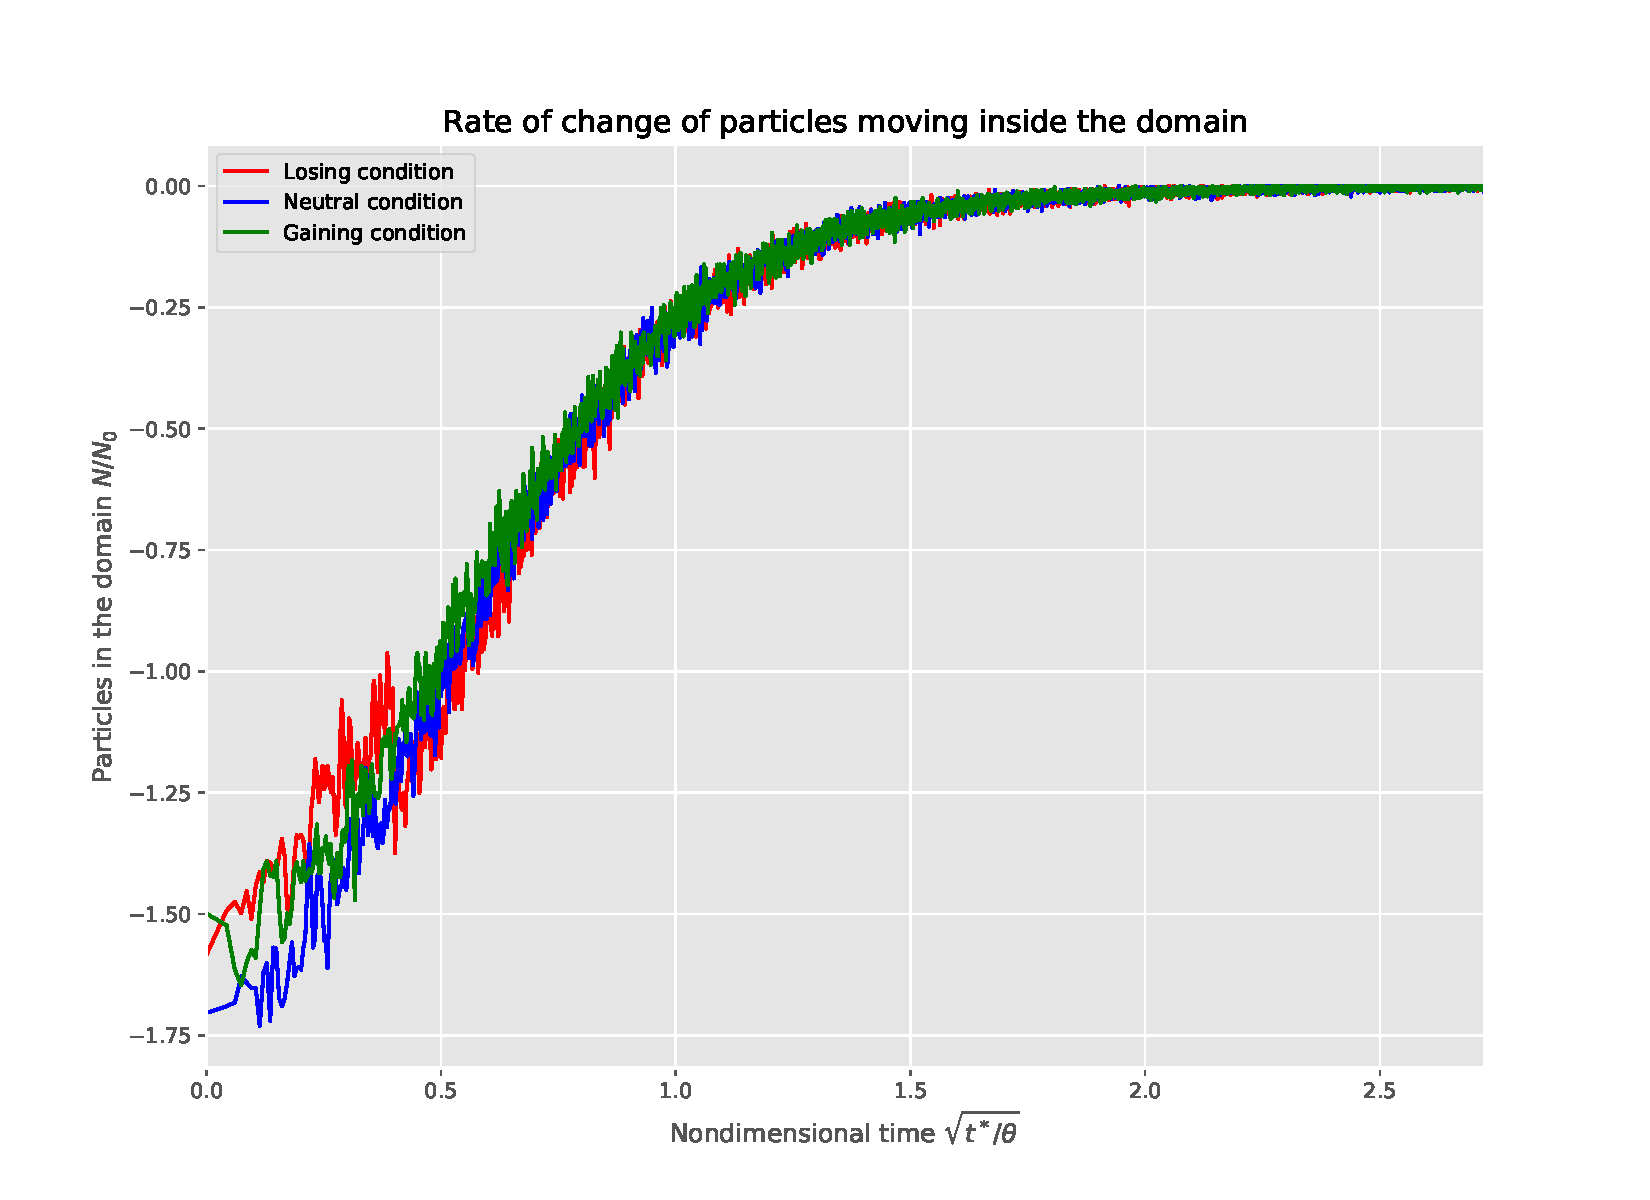
\includegraphics[trim=0.2cm 0.2cm 0.2cm 0.2cm, width=20pc]
{181203_Moving_der.pdf}
\caption{Derivative of moving particles inside the domain}
\label{MOVder}
\end{figure}
% ============================================================================

% 5. COMPARISON BETWEEN NUMERICAL AND EXPERIMENTAL RESULTS FORM FOX'S PAPER
After observing the numerical model results, they are compared with the experimental results from \citet{Fox2018}. In this work the dunes were divided in four locations, each one corresponding to a quarter part of the dune. Therefore, to compare these results with the model, the nondimensional domain is divided in sections with $\pi/2$ width. Then, the experimental results estimated the mean and standard deviation of the mass fraction of clay every $0.5cm$ of depth. 

% ============================================================================
% Comparing with experimental results - figure
\begin{figure}[ht]
\centering
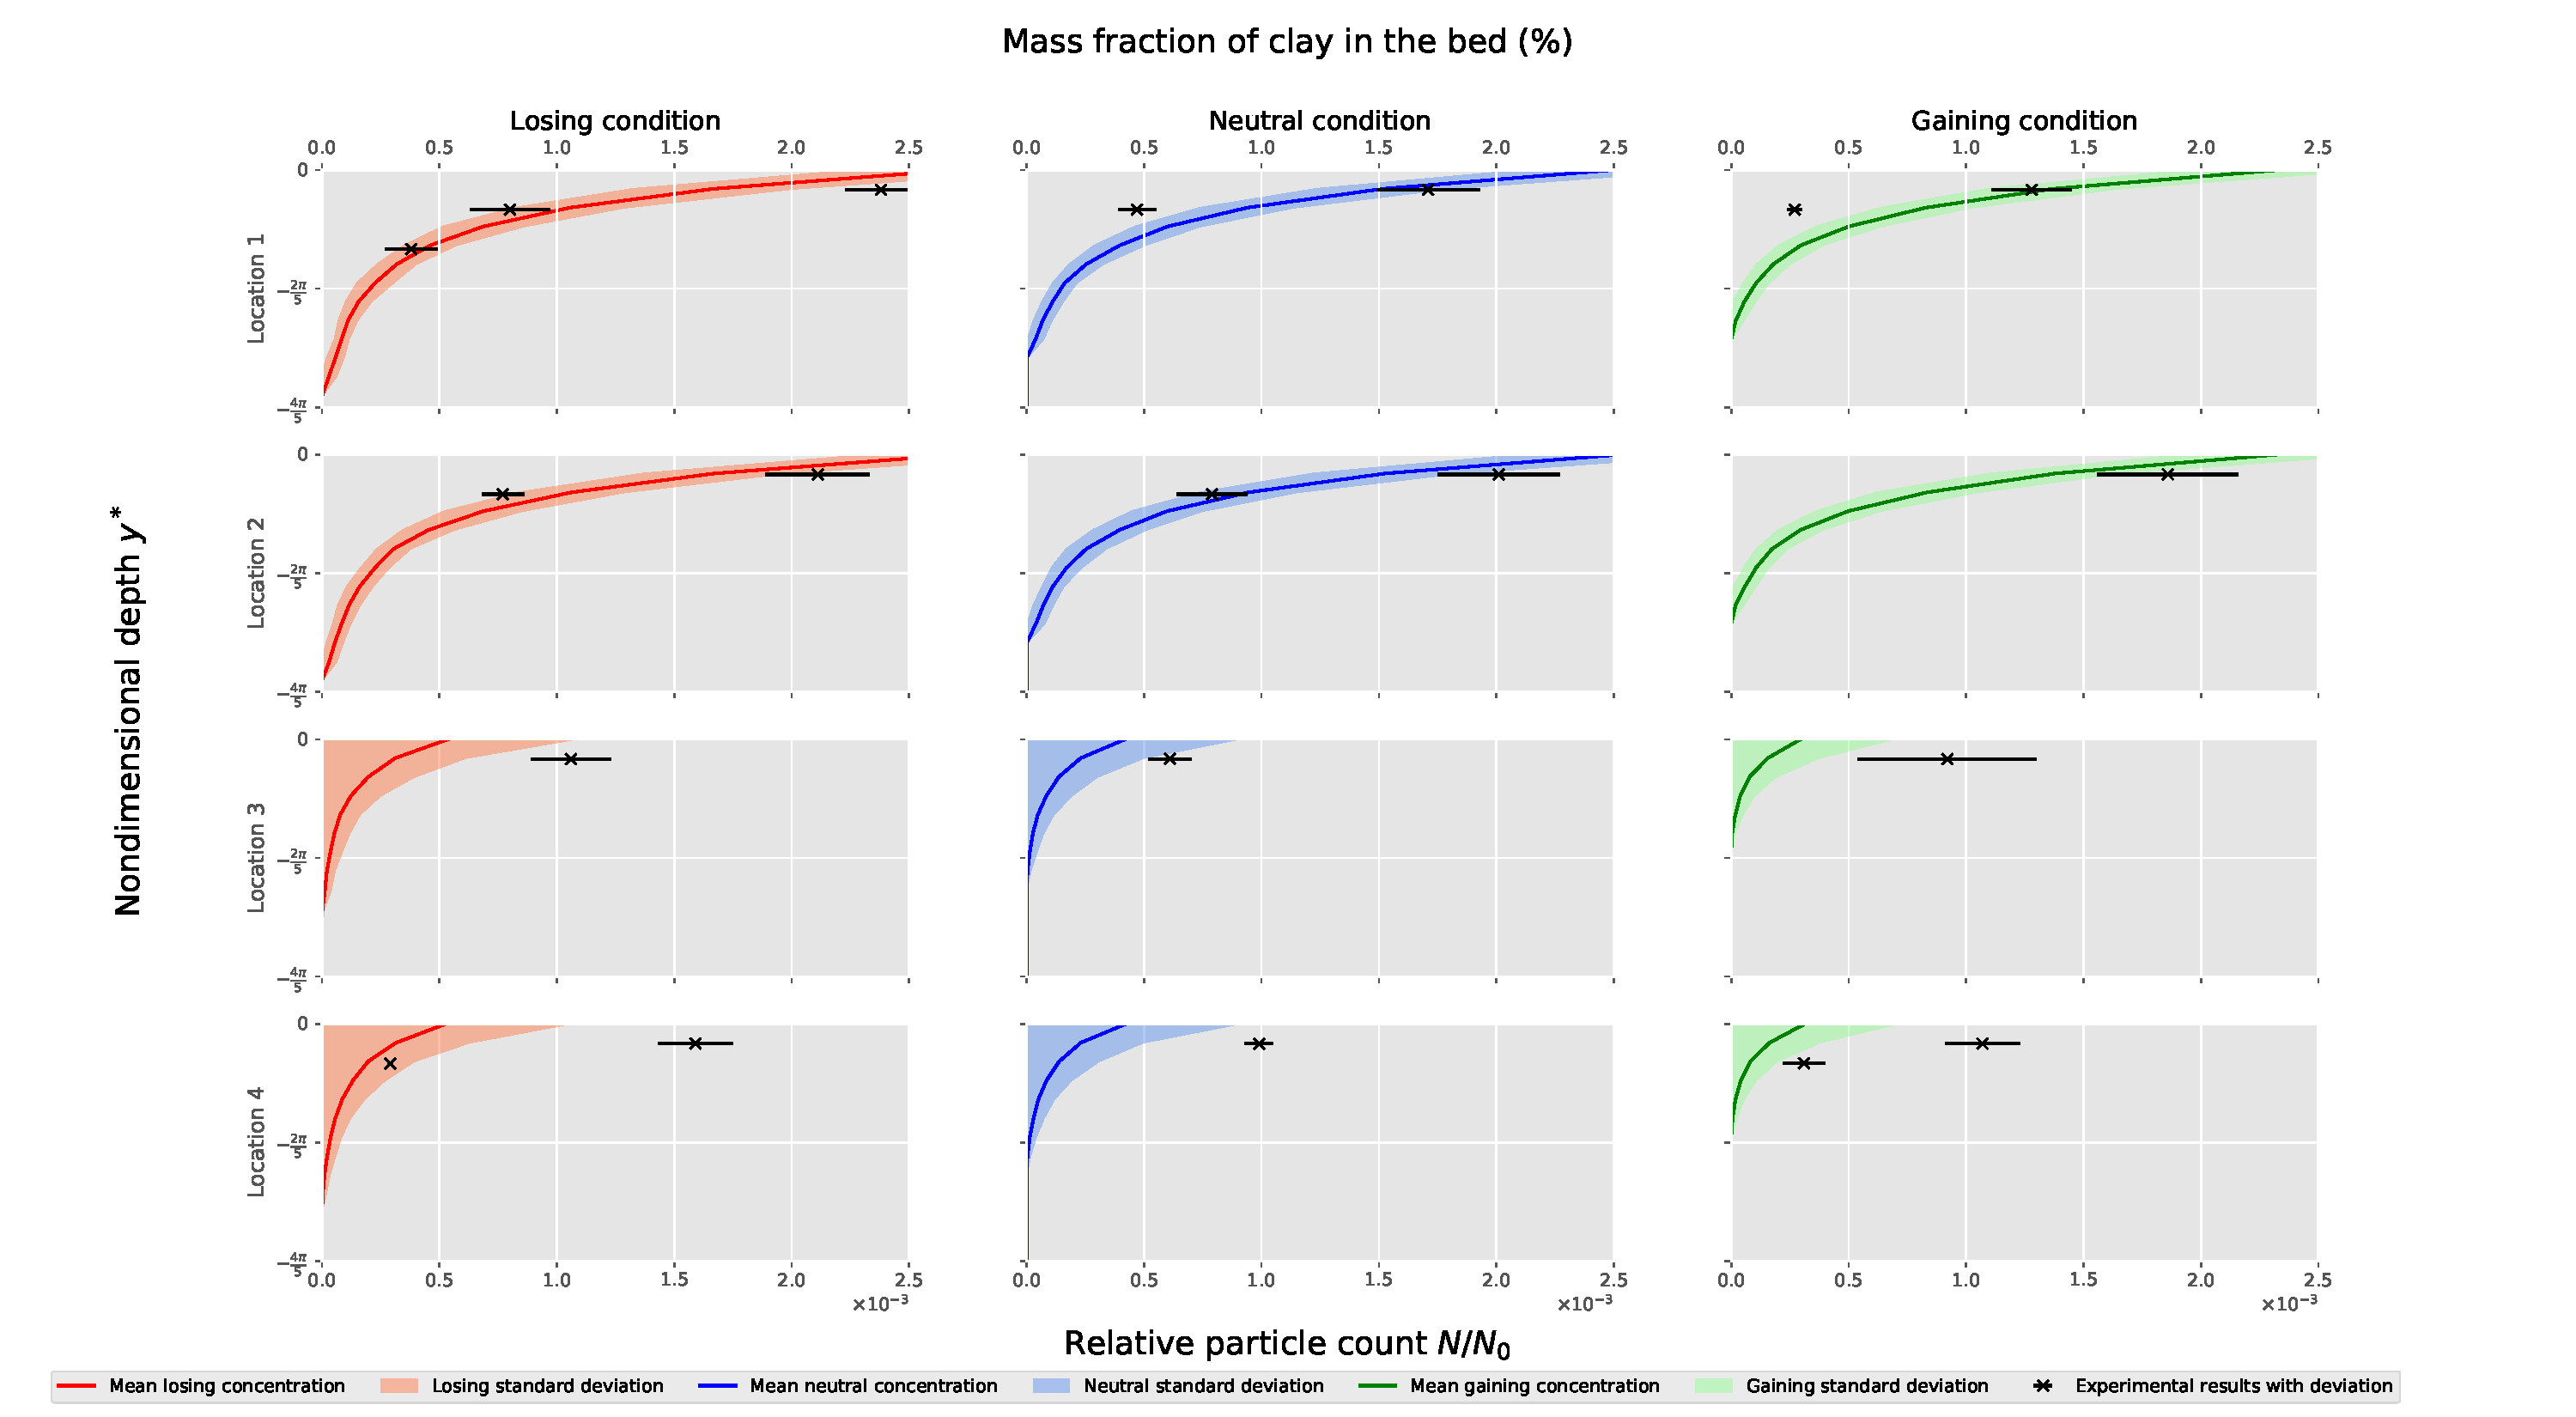
\includegraphics[trim=0.2cm 0.2cm 0.2cm 0.2cm, width=40pc]
{181203_Comparing.pdf}
\caption{Comparison with experimental results from \citep{Fox2018}}
\label{Comparison}
\end{figure}
% ============================================================================

Figure \ref{Comparison} shows the comparison between the experimental results overlayed with the results from the PT model. Black crosses show the mean mass fraction in the depth of reference, and its lines show the plus or minus standard deviation. The scale for these results is shown at the top of figure \ref{Comparison} and it is represented by the percentage of clay mass over total mass of the core extracted. 

Similarly, the colored lines in figure \ref{Comparison} show the mean relative number of particles and the shading shows the standard deviation of this quantity. The scale is located in the bottom part of the figure and it is different than the one used for the experimental results. Nonetheless, both shapes are similar and in a quantitative sense they look similar for the experimental and numerical experiments.

Moreover, clay deposition varies according to the location that is analyzed. In other words, clay tends to deposit more in locations one and two (the stoss side of the dune), and reduces its deposition in locations three and four (lee side of the dune). In fact, the deposition in the latter is provided by the particles that move from right to left in the computational domain following the path lines shown in figure \ref{Velocities}.

Nevertheless, our results show that at locations three and four the PT model is not as good as in locations one and two. In fact, figure \ref{Comparison} shows that for all of the three cases modeled, the experimental results show more clay over depth for locations three and four. That is to say, in the experiments more clay is found inside the domain at the lee side than in the PT model. 

All in all, our results show that there are notable differences between the cases modeled that represent the physics of clay deposition. In addition, they are similar to the experimental results and are able to highlight the contribution of filtration and vertical flow to understand the aforementioned process. 

% ================================================================================
% DISCUSSION SECTION
% ================================================================================
\section{Discussion} \label{Discussion}

% 1. Velocity profiles and deposition patterns analyzed
The proposed PT model combines the use of Langevin's equation and a stochastic filtration framework to simulate clay's deposition in an experimental flume \citep{Li2017}. Indeed, its formulation is simple and straightforward. Moreover, this model does not pose any problems regarding mass conservation, artificial diffusion or unwanted oscillations provoked by numerical scheme instabilities. For the present research, the model was used to assess clay deposition in flumes with static dunes and different vertical flows imposed. 

Although the surface flow conditions are the same, the change in vertical flow conditions reshape the streamlines that are followed by the model's particles. Actually, the Stokes number of an individual particle is so low that we can assume safely that they stick perfectly to the streamlines generated by the velocity profiles. In particular, this assumption is made because of the size of a typical clay particle and the maximum velocity which it is subject to when entering the streambed that is being modeled. 

Stokes number is defined as the relation between the stopping distance and the characteristic length of the phenomenon \citep{Clark2009}. For our model, it was shown in sub subsection \ref{Mathematical_model}. Consequently, the phenomenon of settling velocity is not taken into account as it was in previous works \citep{Packman2000}.

Nevertheless, the PT model is able to capture the physics of the problem. Namely, the velocity profiles shown in figure \ref{Velocities} and the deposition patterns in figures \ref{Heatmap} and \ref{Logmap} show that there are important differences between the conditions modeled. In fact, the gaining flow condition produces less deposition than the neutral and losing condition. Also, deposition is present only at the top of the domain, showing that the model's depth is not relevant for the phenomenon of clay deposition since it deposits at the top and there is no particle penetration to deep parts of the domain. 

Moreover, the logarithmic deposition patterns shown in figure \ref{Logmap} show that a change in the vertical flow conditions affect not only the maximum penetration depth of the clay, but also spread more evenly in the horizontal direction the clay particles that are modeled. In that sense, clay presence in the streambed will cover more dune's width in the losing condition and it will be discontinuous in the neutral and gaining cases. In effect, this explains the decay hyporheic exchange in the experiments run with conservative tracers after clay injections under different vertical flow conditions \citep{Fox2014,Fox2018}.

In addition, the PT model shows that the velocity profiles and filtration produce an uneven distribution of clay in the pore scale. In other words, clay penetration is stratified, but there are spots with no particles in different depths independently of the condition modeled. Despite this, it is evident that these spots with no particles are more persistent in the cases of neutral and gaining conditions. Our results suggest agreement with experimental results that clearly show an uneven distribution of clay mass in the dunes where the cores were extracted \citep{Fox2018}.

As respects to the comparison made in figure \ref{Comparison}, our results suggest that the PT model is able to simulate clay deposition in a single dune with similar results to the experiments. Indeed, the decay in clay concentration with depth is similar to the experimental results presented by \citet{Fox2018}, suggesting that the PT model grasps the physical processes of clay deposition in sand beds. However, regarding the standard deviation of clay's mass fraction is not as accurate as expected. This can be explained by the difference in shape of the dunes in the experiment and the proposed dune for the numerical model. In fact, this difference highlights the difficulty that any numerical model has when simulating heterogeneous media and complex phenomena.  

% 2. Discussion about the particle's behavior over time (remobiliztion, RTF and what does that imply in the context of clay deposition)
Regarding the behavior of particles over time, the differences between vertical flow conditions are also noticeable in figures \ref{Pvst} and \ref{RTF}. For example, it is clear that particles tend to be remobilized easily when there is the presence of a gaining flow. In fact, the total remobilized particles between cases ranges from 0.18 in the losing condition to almost 0.3 in the gaining scenario (units in fraction of particles). Namely, remobilized particles almost double when passing from the losing to the gaining case. This result suggests that the clay concentration decay in a flume with clay mixed will be lower for gaining conditions than for neutral or losing conditions, as shown by \citet{Fox2018}.

In particular, for the particles' filtering, our results suggest that the vertical flow conditions play a crucial role in affecting this process. Granted that the filtering coefficient is the same for all of the modeled scenarios, it is undeniable that particle filtering is fostered by losing flow conditions. That is, the more negative the vertical velocity is, the more a particle is going to travel in the streambed, and therefore will be more prone to be subject to filtering during the simulation. 

Furthermore, the rate of change of the RTF shown in figure \ref{RTFder} suggests that the particles' movement and retention inside the domain depends also on the imposed flow conditions and not just on the filtration coefficient. In fact, the curves of figure \ref{RTFder} and \ref{MOVder} are almost identical, suggesting that the filtration process is the same for all of the modeled cases and that the initial remobilization caused by the imposed flow condition is the main driver of the phenomenon analyzed. 

Consequently, in all of the cases the main difference is set at the initial times of the simulations, where particles are remobilized according to the imposed vertical velocity. In fact, particles that are not remobilized at early times are subject to movement or filtration, and the more particles are moving inside the domain (losing condition), the more the filtration process will act during the simulation. 

In general, our model shows that clay deposition is a phenomenon that results from the combination of the velocity inside the streambed, the vertical flow condition (losing, neutral or gaining), and the filtering properties of the material. In order of importance, the filtering part of the model enforces the stopping of clay particles inside the porous matrix. However, this process is fostered and changed drastically when a vertical flow is imposed. 

% ================================================================================
% CONCLUSIONS SECTION
% ================================================================================
\section{Conclusions} \label{Conclusions}

The PT model implemented and presented in this paper combines the physical description of the colloid movement with the probabilistic framework of the filtration of the clay particles inside a characteristic dune of an experimental flume. Namely, these models are more suitable to represent phenomena that is not described accurately with the ADE \citep{Noetinger2016}. Moreover, their results are straightforward to interpret since all of the calculations are made with the number of particles inside the computational domain. 

Also, the implemented model represents the physical phenomenon coherently. Indeed, mass conservation is ensured at all time, there is no artificial diffusion (especially numerical diffusion), and the results are comparable with experimental set-ups from previous works. Nonetheless, the numerical simulation can assess different results and highlight important features that the experiments cannot recognize. 

Regarding these features, our model shows clearly that the vertical flow conditions imposed are responsible for the differences in deposition patterns and amount of clay inside the domain. Similarly, the filtration phenomenon will act as a control of particles inside the domain. Consequently, when in the presence of gaining flow condition, the amount of particles inside the domain will be less than in the other two cases, while the rate at which particles are filtered inside the domain is the same for all of the three modeled cases.

In particular, our model's most important finding is that vertical flow condition is independent from filtration of particles inside the domain. Therefore, the differences in deposition patterns, maximum penetration depth and the steady final value of the RTF are caused only by vertical velocities imposed as losing/gaining conditions. On the other hand, filtration coefficient is responsible for the time that takes to the RTF to get to a constant value after the first injection. Put differently, vertical flow conditions imposed relocate particles and remobilize particles out of the domain in different amounts and account for the difference between the three cases modeled.

As regards to remobilization, this phenomenon is relevant only for a brief time of every one of our models, but its presence and the return of particles from the SWI to the free stream clearly depend also on the vertical flow conditions imposed. In other words, remobilization is not connected with filtration, but it rather works side by side with it to determine the shape of the residence time function for the different cases modeled. 

In the direction of test further our numerical model, more experimental results are needed to assess our PT model. In addition, future work aims to represent changes in permeability due to clay's deposition since it is evident that an important clay deposition will hinder porosity and hence permeability and hydraulic conductivity of the media. 

To conclude, the PT framework is suitable to study phenomena that is difficultly modeled by continuum mechanics equation such as ADE. Their flexibility allows to model phenomena in small scale $O(10^{-1}m)$ to reach scale $O(10^3-10^4 m)$ with results that are comparable to experimental or field study results.  

\acknowledgments
We thank Zuckerberg Institute for Water Research, The J. Blaustein Institutes for Desert Research, Ben-Gurion University of the Negev (Beersheba, Israel), for providing the experimental data for comparisons; and the Water Research Group at Northwestern University for providing the basis for the particle-tracking model. Supporting data available at ...... Authors declare no conflicts of interest.

% References and Citations
\bibliography{APR_Refs.bib}

% % FIGURE IN THE END OF THE DOCUMENT TO MATCH DRAFT SUBMISSION

% % ============================================================================
% % Conceptual model of the problem proposed - figure
% \begin{figure}[ht]
% \centering
% \includegraphics[clip, trim=4.2cm 4.5cm 8cm 3cm, width=18pc]
% {1807010Conceptual.pdf}
% \caption{Conceptual model for the posed problem}
% \label{Conceptual}
% \end{figure}
% % ============================================================================

% % ============================================================================
% % TABLE WITH PHYSICAL AND NUMERICAL PARAMETERS FOR THE PARTICLE-TRACKING
% % MODEL THAT WAS PROPOSED
% % ============================================================================
% \begin{table}
% \caption{Physical \citep{Fox2018} and numerical parameters \citep{Packman2000}
% for the particle-tracking model. }
% \label{TF:Phys_Param}
% \centering
% \begin{tabular}{l c c}
% \hline
% PHYSICAL PARAMETERS						& SYMBOL			& VALUE			\\
% \hline
%   Flume width $[cm]$  					& $W$				& 29.0 			\\
%   Sediment porosity $[-]$				& $\theta$			& 0.33 			\\
%   Hydraulic conductivity $[cm/s]$ 		& $K$				& 0.12 			\\
%   Flow $[l/min]$						& $Q$				& 261.0			\\
%   Mean stream velocity $[cm/s]$			& $U$				& 15.0 			\\
%   Streambed depth $[cm]$				& $d_b$				& 20.0 			\\
%   Dune wavelegth $[cm]$					& $\lambda$			& 15.0 			\\
%   Water depth $[cm]$					& $d$				& 8.8 			\\
%   Total streambed area $[cm^{2}]$		& $A$				& 15.1	 		\\
%   Inflow/Outflow$^{b}$ $[cm/d]$			& $q_{in}$			& $\pm 12.5$	\\
%   Filtering coefficient $[1/cm]$		& $\lambda_f$		& 0.6			\\
% \hline
% NUMERICAL PARAMETERS					& 					& 				\\
% \hline
%   Number of particles $[-]$				& $n$				& 1.0E5			\\
%   Real time simulated $[min]$			& $T$				& 60.0 			\\
%   Number of timesteps per simulation $[-]$ &$nT$			& 1.0E4			\\
%   Horzontal particle offset $[-]$		& $x_{off}$			& 1.0E-3		\\
%   Vertical particle offset $[-]$		& $y_{off}$			& $100*eps^{c}$ \\
% \hline
% \multicolumn{2}{l}{$^{a}$All units in $cgs$ system for convenience} \\
% \multicolumn{2}{l}{$^{b}$Positive quantities point upwards, negative 
% downwards} \\
% \multicolumn{2}{l}{$^{c}$Machine precision}
% \end{tabular}
% \end{table}
% % ============================================================================

% % ============================================================================
% % Velocity profiles - figure
% \begin{figure}[ht]
% \centering
% \includegraphics[trim=2cm 1.5cm 4cm 0.1cm, width=25pc]
% {181203_Streamlines.pdf}
% \caption{Streamlines under different vertical flow conditions: (A) Losing, (B) Neutral and (C) Gaining. Plots' domains are shifted from $[0, 2 \pi]$ to $[-\pi /2, \pi/2]$ since domain is periodic. Note that the vertical scale is distorted.}
% \label{Velocities}
% \end{figure}
% % ============================================================================

% % ============================================================================
% % Numerical model of the problem proposed - figure
% \begin{figure}[ht]
% \centering
% \includegraphics[clip, trim=4.2cm 4.5cm 8cm 3cm, width=18pc]
% {181129Numerical.pdf}
% \caption{Depiction of numerical model proposed}
% \label{Numerical}
% \end{figure}
% % ============================================================================

% % ============================================================================
% % Concentration map - figure
% \begin{figure}[ht]
% \centering
% \includegraphics[trim=0.2cm 0.2cm 0.2cm 0.2cm, width=45pc]
% {181203_Concentrations.pdf}
% \caption{Particle deposition in different times (rows), and under different inflow/outflow conditions (columns) (Note that axis are not to scale).}
% \label{Heatmap}
% \end{figure}
% % ============================================================================

% % ============================================================================
% % Logarithm of concentration - figure
% \begin{figure}[ht]
% \centering
% \includegraphics[trim=0.2cm 0.2cm 0.2cm 0.2cm, width=45pc]
% {181203_Logplot.pdf}
% \caption{Logarithm of particle deposition in different times (rows), and under different inflow/outflow conditions (columns) (Note that axis are not to scale).}
% \label{Logmap}
% \end{figure}
% % ============================================================================

% % ============================================================================
% % Particles in time - figure
% \begin{figure}[ht]
% \centering
% \includegraphics[trim=0.2cm 0.2cm 0.2cm 0.2cm, width=35pc]
% {181203_Pvst.pdf}
% \caption{Particle's behavior over time. A. Losing condition. B. Neutral condition and C. Gaining condition}
% \label{Pvst}
% \end{figure}
% % ============================================================================

% % ============================================================================
% % Residence time function - figure
% \begin{figure}[ht]
% \centering
% \includegraphics[trim=0.2cm 0.2cm 0.2cm 0.2cm, width=20pc]
% {181203_RTF.pdf}
% \caption{Residence time function for different flow conditions imposed}
% \label{RTF}
% \end{figure}
% % ============================================================================

% % ============================================================================
% % RTF der - figure
% \begin{figure}[ht]
% \centering
% \includegraphics[trim=0.2cm 0.2cm 0.2cm 0.2cm, width=20pc]
% {181203_RTF_der.pdf}
% \caption{Derivative of RTF for the three conditions}
% \label{RTFder}
% \end{figure}
% % ============================================================================

% % ============================================================================
% % Moving der - figure
% \begin{figure}[ht]
% \centering
% \includegraphics[trim=0.2cm 0.2cm 0.2cm 0.2cm, width=20pc]
% {181203_Moving_der.pdf}
% \caption{Derivative of moving particles inside the domain}
% \label{MOVder}
% \end{figure}
% % ============================================================================

% % ============================================================================
% % Comparing with experimental results - figure
% \begin{figure}[ht]
% \centering
% \includegraphics[trim=0.2cm 0.2cm 0.2cm 0.2cm, width=40pc]
% {181203_Comparing.pdf}
% \caption{Comparison with experimental results from \citep{Fox2018}}
% \label{Comparison}
% \end{figure}
% % ============================================================================

\end{document}

% ================================================================================
% GUIDELINES (delete when submitting)
% ================================================================================

%Text here ===>>>

%%

%  Numbered lines in equations:
%  To add line numbers to lines in equations,
%  \begin{linenomath*}
%  \begin{equation}
%  \end{equation}
%  \end{linenomath*}

%% Enter Figures and Tables near as possible to where they are first mentioned:
%
% DO NOT USE \psfrag or \subfigure commands.
%
% Figure captions go below the figure.
% Table titles go above tables;  other caption information
%  should be placed in last line of the table, using
% \multicolumn2l{$^a$ This is a table note.}
%
%----------------
% EXAMPLE FIGURE
%
% \begin{figure}[h]
% \centering
% when using pdflatex, use pdf file:
% \includegraphics[width=20pc]{figsamp.pdf}
%
% when using dvips, use .eps file:
% \includegraphics[width=20pc]{figsamp.eps}
%
% \caption{Short caption}
% \label{figone}
%  \end{figure}
%
% ---------------
% EXAMPLE TABLE
%
% \begin{table}
% \caption{Time of the Transition Between Phase 1 and Phase 2$^{a}$}
% \centering
% \begin{tabular}{l c c}
% \hline
%  Run  & Time (min) & hola  \\
% \hline
%   $l1$  & 260 & 500  \\
%   $l2$  & 300 & 500  \\
%   $l3$  & 340 & 500  \\
%   $h1$  & 270 & 500  \\
%   $h2$  & 250 & 500  \\
%   $h3$  & 380 & 500  \\
%   $r1$  & 370 & 500  \\
%   $r2$  & 390 & 500  \\
% \hline
% \multicolumn{3}{l}{$^{a}$Footnote text here.}
% \end{tabular}
% \end{table}

%% SIDEWAYS FIGURE and TABLE
%% AGU prefers the use of {sidewaystable} over {landscapetable} as it causes 
%% fewer problems.
%
% \begin{sidewaysfigure}
% \includegraphics[width=20pc]{figsamp}
% \caption{caption here}
% \label{newfig}
% \end{sidewaysfigure}
%
%  \begin{sidewaystable}
%  \caption{Caption here}
% \label{tab:signif_gap_clos}
%  \begin{tabular}{ccc}
% one&two&three\\
% four&five&six
%  \end{tabular}
%  \end{sidewaystable}

%% If using numbered lines, please surround equations with 
%% \begin{linenomath*}...\end{linenomath*}
% \begin{linenomath*}
% \begin{equation}
% y|{f} \sim g(m, \sigma),
% \end{equation}
% \end{linenomath*}

%%% End of body of article

%%%%%%%%%%%%%%%%%%%%%%%%%%%%%%%%
%% Optional Appendix goes here
%
% The \appendix command resets counters and redefines section heads
%
% After typing \appendix
%
%\section{Here Is Appendix Title}
% will show
% A: Here Is Appendix Title
%
%\appendix
%\section{Here is a sample appendix}

%%%%%%%%%%%%%%%%%%%%%%%%%%%%%%%%%%%%%%%%%%%%%%%%%%%%%%%%%%%%%%%%
%
% Optional Glossary, Notation or Acronym section goes here:
%
%%%%%%%%%%%%%%
% Glossary is only allowed in Reviews of Geophysics
%  \begin{glossary}
%  \term{Term}
%   Term Definition here
%  \term{Term}
%   Term Definition here
%  \term{Term}
%   Term Definition here
%  \end{glossary}

%
%%%%%%%%%%%%%%
% Acronyms
%   \begin{acronyms}
%   \acro{Acronym}
%   Definition here
%   \acro{EMOS}
%   Ensemble model output statistics
%   \acro{ECMWF}
%   Centre for Medium-Range Weather Forecasts
%   \end{acronyms}

%
%%%%%%%%%%%%%%
% Notation
%   \begin{notation}
%   \notation{$a+b$} Notation Definition here
%   \notation{$e=mc^2$}
%   Equation in German-born physicist Albert Einstein's theory of special
%  relativity that showed that the increased relativistic mass ($m$) of a
%  body comes from the energy of motion of the body—that is, its kinetic
%  energy ($E$)—divided by the speed of light squared ($c^2$).
%   \end{notation}




%%%%%%%%%%%%%%%%%%%%%%%%%%%%%%%%%%%%%%%%%%%%%%%%%%%%%%%%%%%%%%%%
%
%  ACKNOWLEDGMENTS
%
% The acknowledgments must list:
%
% >>>>	A statement that indicates to the reader where the data
% 	supporting the conclusions can be obtained (for example, in the
% 	references, tables, supporting information, and other databases).
%
% 	All funding sources related to this work from all authors
%
% 	Any real or perceived financial conflicts of interests for any
%	author
%
% 	Other affiliations for any author that may be perceived as
% 	having a conflict of interest with respect to the results of this
% 	paper.
%
%
% It is also the appropriate place to thank colleagues and other contributors.
% AGU does not normally allow dedications.

% This part is taken from recent papers with acknowledgement

More Information and Advice:

%% ------------------------------------------------------------------------ %%
%  SECTION HEADS
%% ------------------------------------------------------------------------ %%

% Capitalize the first letter of each word (except for
% prepositions, conjunctions, and articles that are
% three or fewer letters).

% AGU follows standard outline style; therefore, there cannot be a section 1 without
% a section 2, or a section 2.3.1 without a section 2.3.2.
% Please make sure your section numbers are balanced.
% ---------------
% Level 1 head
%
% Use the \section{} command to identify level 1 heads;
% type the appropriate head wording between the curly
% brackets, as shown below.
%
%An example:
%\section{Level 1 Head: Introduction}
%
% ---------------
% Level 2 head
%
% Use the \subsection{} command to identify level 2 heads.
%An example:
%\subsection{Level 2 Head}
%
% ---------------
% Level 3 head
%
% Use the \subsubsection{} command to identify level 3 heads
%An example:
%\subsubsection{Level 3 Head}
%
%---------------
% Level 4 head
%
% Use the \subsubsubsection{} command to identify level 3 heads
% An example:
%\subsubsubsection{Level 4 Head} An example.
%
%% ------------------------------------------------------------------------ %%
%  IN-TEXT LISTS
%% ------------------------------------------------------------------------ %%
%
% Do not use bulleted lists; enumerated lists are okay.
% \begin{enumerate}
% \item
% \item
% \item
% \end{enumerate}
%
%% ------------------------------------------------------------------------ %%
%  EQUATIONS
%% ------------------------------------------------------------------------ %%

% Single-line equations are centered.
% Equation arrays will appear left-aligned.

Math coded inside display math mode \[ ...\]
 will not be numbered, e.g.,:
 \[ x^2=y^2 + z^2\]

 Math coded inside \begin{equation} and \end{equation} will
 be automatically numbered, e.g.,:
 \begin{equation}
 x^2=y^2 + z^2
 \end{equation}


% To create multiline equations, use the
% \begin{eqnarray} and \end{eqnarray} environment
% as demonstrated below.
\begin{eqnarray}
  x_{1} & = & (x - x_{0}) \cos \Theta \nonumber \\
        && + (y - y_{0}) \sin \Theta  \nonumber \\
  y_{1} & = & -(x - x_{0}) \sin \Theta \nonumber \\
        && + (y - y_{0}) \cos \Theta.
\end{eqnarray}

%If you don't want an equation number, use the star form:
%\begin{eqnarray*}...\end{eqnarray*}

% Break each line at a sign of operation
% (+, -, etc.) if possible, with the sign of operation
% on the new line.

% Indent second and subsequent lines to align with
% the first character following the equal sign on the
% first line.

% Use an \hspace{} command to insert horizontal space
% into your equation if necessary. Place an appropriate
% unit of measure between the curly braces, e.g.
% \hspace{1in}; you may have to experiment to achieve
% the correct amount of space.

%% ------------------------------------------------------------------------ %%
%  EQUATION NUMBERING: COUNTER
%% ------------------------------------------------------------------------ %%

% You may change equation numbering by resetting
% the equation counter or by explicitly numbering
% an equation.

% To explicitly number an equation, type \eqnum{}
% (with the desired number between the brackets)
% after the \begin{equation} or \begin{eqnarray}
% command.  The \eqnum{} command will affect only
% the equation it appears with; LaTeX will number
% any equations appearing later in the manuscript
% according to the equation counter.
%

% If you have a multiline equation that needs only
% one equation number, use a \nonumber command in
% front of the double backslashes (\\) as shown in
% the multiline equation above.

% If you are using line numbers, remember to surround
% equations with \begin{linenomath*}...\end{linenomath*}

%  To add line numbers to lines in equations:
%  \begin{linenomath*}
%  \begin{equation}
%  \end{equation}
%  \end{linenomath*}

% Please use ONLY \citet and \citep for reference citations.
% DO NOT use other cite commands (e.g., \cite, \citeyear, \nocite, \citealp, etc.).
%% Example \citet and \citep:
%  ...as shown by \citet{Boug10}, \citet{Buiz07}, \citet{Fra10},
%  \citet{Ghel00}, and \citet{Leit74}.

%  ...as shown by \citep{Boug10}, \citep{Buiz07}, \citep{Fra10},
%  \citep{Ghel00, Leit74}.

%  ...has been shown \citep [e.g.,][]{Boug10,Buiz07,Fra10}.